\chapter{Behaviour of a Concurrent System}
When we analyze a concurrent system, we are looking at its behavior, which can be viewed in two primary ways: as a set of traces (histories of what has happened) or as a set of traces plus a branching structure. The branching structure is crucial because it accounts for the points at which a system makes a choice between different possible futures. 

\begin{figure}[ht]
    \centering
    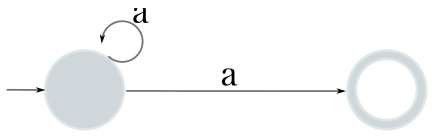
\includegraphics[width=0.4\linewidth]{images/process-behaviour.png}
    \caption{Concurrent system as a set of traces and branching structure.}
    \label{fig:process-behaviour}
\end{figure}

\section{Finite Automata}
In traditional formal language theory, a \textit{finite non-deterministic automaton}\index{finite non-deterministic automaton} is defined as a quintuple $M=(Q,Act,q_0,F,T)$, where:
\begin{itemize}
    \item $Q$ is the set of states. 
    \item $Act$ is the set of actions. 
    \item $q_0$ is the starting state.
    \item $F$ is the set of final states.
    \item $T$ is the transition relation, where $T\subseteq Q\times Act\times Q$. 
\end{itemize}
    
Under this view, the behavior of an automaton is characterized by language equivalence. The language $L(M)$ is the set of all sequences of input characters (traces) that lead the automaton from its starting state to a final state. Formally, two automata $M_1$ and $M_2$ are considered equivalent if and only if $L(M_1)=L(M_2)$.

Language equivalence is often too "coarse" for concurrency theory because it ignores the branching structure of a process. Consider two vending machine (Figure \ref{fig:vending-machines}) implementations that both deliver tea for 20 cents or coffee for 40 cents. 

\begin{figure}[ht]
    \centering
    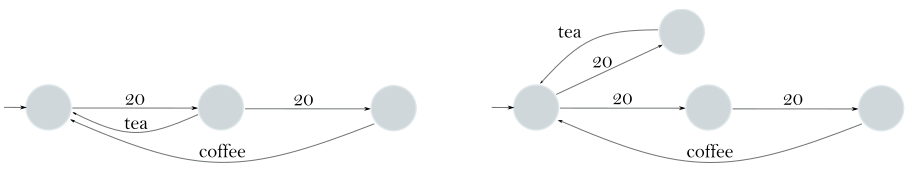
\includegraphics[width=1\linewidth]{images/vending-machines.png}
    \caption{Two vending machines for coffee and tea.}
    \label{fig:vending-machines}
\end{figure}

\begin{itemize}
    \item Machine 1: After inserting the first 20 cents, the user can choose to take tea or insert another 20 cents for coffee. 
    \item Machine 2: Upon receiving the first 20 cents, the machine internally decides whether it will provide tea or wait for another 20 cents for coffee.
\end{itemize}

Both machines generate the same language of traces: $(20.(tea+20.coffee))*$. However, from the perspective of an external observer (the user), they behave differently. In the second machine, the user might insert 20 cents and find they cannot choose tea because the machine has already non-deterministically branched toward the "coffee" path. 

\begin{figure}[ht]
    \centering
    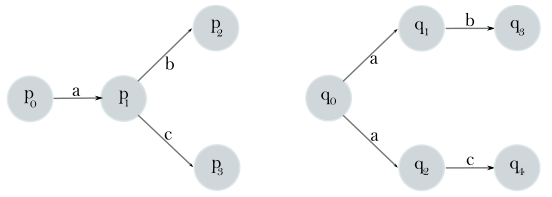
\includegraphics[width=0.7\linewidth]{images/determinism-non-determinism.png}
    \caption{Determinism vs. non-determinism.}
    \label{fig:determinism-non-determinism}
\end{figure}

The essence of the difference is when the decision to branch is taken. Language equivalence "forgets" these branching points, making it an insufficient tool for describing interactive processes.

\section{Labeled Transition Systems (LTS)}
To better model concurrency, we use \textit{Labeled Transition Systems (LTS)}\index{Labeled Transition Systems} instead of finite automata.  While they appear similar, there are three fundamental differences:
\begin{enumerate}
    \item \textit{Infinite States:} Automata usually have a finite number of states, but an LTS can have an infinite state space.
    \item \textit{Initial States:} An automaton has one fixed starting state, whereas in an LTS, every state can be treated as a potential starting point for a behavior.
    \item \textit{Final States:} Automata use final states to define an accepted language. In an LTS, this notion is not very informative because we are interested in the ongoing interaction rather than just terminal acceptance. 
\end{enumerate}

\begin{Definition}{Labeled Transition Systems (LTS)}{}
A Labeled Transition System is a pair $(Q,T)$, where $Q$ is the set of states and $T$ is the transition relation $T\subseteq Q\times N\times Q$, with $N$ being a fixed set of action names. We write $s\xrightarrow{a}s'$ to indicate that state $s$, after performing action $a$, evolves into state $s'$.
\end{Definition}

\section{Bisimulation}
We need a notion of equivalence that captures the "step-by-step" behavior of processes. Intuitively, two states are equivalent if they can perform the same actions and reach states that are themselves equivalent. 
For example, in Figure \ref{fig:determinism-non-determinism} $P_0$ and $Q_0$ are different because, after an $a$, the left process can decide to do $b$ or $c$, whereas the right process must decide this before performing $a$.

\begin{Definition}{Simulation}{}
Let $(Q,T)$ be an LTS. A binary relation $S\subseteq Q\times Q$ is a \textit{simulation}\index{simulation} if and only if:
\begin{equation*}
    \forall(p,q)\in S,\forall p\xrightarrow{a}p',\exists q\xrightarrow{a}q' \textit{ such that } (p',q')\in S
\end{equation*}
\end{Definition}

We say $p$ is simulated by $q$ if such a relation exists. In our vending machine example, a deterministic machine might be simulated by a non-deterministic one, but not vice versa, because the non-deterministic machine might reach a state where it can no longer perform an action the deterministic one could. 

\begin{Definition}{Bisimulation}{}
A relation $S$ is a \textit{bisimulation}\index{bisimulation} if both $S$ and its inverse $S^{-1}$ are simulations. Two states $p$ and $q$ are bisimilar (written $p\sim q$) if there exists a bisimulation $S$ such that $(p,q)\in S$.
\end{Definition}

Bisimulation is defined on the states of a single LTS. To compare states from two different systems, we simply take the disjoint union of the two LTSs and treat them as one.

For example, in the LST of Figure \ref{fig:determinism-non-determinism}, $q_0$ is simulated by $p_0$ is shown by the following simulation relation:
\begin{equation*}
     S = \{(q_0,p_0), (q_1,p_1), (q_2,p_1), (q_3,p_2), (q_4,p_3)\}
\end{equation*}

To let $p_0$ be simulated by $q_0$, we should have that $p_1$ is simulated by $q_1$ or $q_2$. If $S$ contained one among $(p_1,q_1)$ or $(p_1,q_2)$, then it would not be a simulation:
indeed, $p_1$ can perform both a $c$ (whereas $q_1$ cannot) and a $b$ (whereas $q_2$ cannot).

It is important to note that simply having $p$ simulate $q$ and $q$ simulate $p$ (through two different relations) does not mean $p$ and $q$ are bisimilar. Bisimilarity requires a single relation to work in both directions.

\begin{figure}[ht]
    \centering
    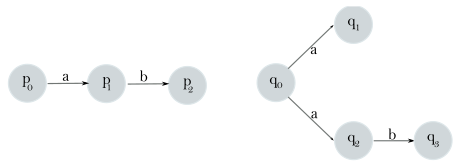
\includegraphics[width=0.7\linewidth]{images/not-sim-is-bisim.png}
    \caption{Simulation that is not enough for Bisimulation.}
    \label{fig:not-sim-is-bisim}
\end{figure}

For example, in the LTS of Figure \ref{fig:not-sim-is-bisim}, we might find that $p_0$ is simulated by $q_0$ via relation:
\begin{equation*}
    S = \{(p_0, q_0), (p_1, q_2), (p_2, q_3)\}
\end{equation*}
and $q_0$ is simulated by $p_0$ via relation:
\begin{equation*}
    S' =\{(q_0,p_0),(q_1,p_1),(q_2,p_1),(q_3,p_2)\}
\end{equation*}
However, $p_0$ and $q_0$ are not bisimilar: the transition $q_0\xrightarrow{a}q_1$ is not bisimulable by any transition from $p_0$. Indeed, $p_0\xrightarrow{a}p_1$ does not suffice, because $p_1$ can perform a $b$ and so cannot be bisimilar to $q_1$.

\begin{figure}[ht]
    \centering
    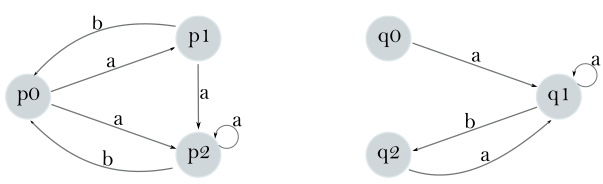
\includegraphics[width=0.7\linewidth]{images/example-bisim.png}
    \caption{An example of bisimilarity.}
    \label{fig:example-bisim}
\end{figure}

Now let's consider the relation in Figure \ref{fig:example-bisim}. To prove $p_0\sim q_0$, we must construct a specific relation $S$ and show it is a bisimulation.
\begin{align*}
    S &= \{(p_0,q_0), (p_1,q_1), (p_2,q_1), (p_0,q_2)\}\\
    S^{-1} &= \{(q_0,p_0), (q_1,p_1), (q_1,p_2), (q_2,p_0)\}
\end{align*}

To verify this:
\begin{enumerate}
    \item Check that for every pair in $S$, any action from the first state can be matched by the second to a pair still in $S$. 
    \item Check that $S^{-1}$ also satisfies this property.
\end{enumerate}

\subsection{Properties of Bisimilarity}
Bisimilarity ($\sim$) is the fundamental tool for relating process behaviors. It possesses several mathematical properties that make it robust.

\begin{Thm}{Bisimilarity is an Equivalence Relation}{}
\begin{enumerate}
    \item \textit{Reflexivity ($q\sim q$):} The identity relation $Id=\{(p,p):p\in Q\}$ is a bisimulation (it is a simulation, as well as its inverse - i.e. $S$ itself).
    \item \textit{Symmetry ($p\sim q\implies q\sim p$):} If $S$ is a bisimulation containing $(p,q)$ then, by definition of bisimulation, $S^{-1}$ is a bisimulation containing $(q,p)$.
    \item \textit{Transitivity ($p\sim q\land q\sim r\implies p\sim r$):} If $S_1$ and $S_2$ are bisimulations, their composition $S = \{(x, z) : \exists y \text{ s.t. } (x, y) \in S_1 \land (y, z) \in S_2\}$ is also a bisimulation.

    Let $(x, z) \in S$ and $x\xrightarrow{a}x'$. If $(x, z)$ belongs to $S$, then, by definition, there exists $y$ such that $(x,y) \in S_1$ and $(y,z) \in S_2$. Since $S_1$ is a bisimulation, there exists $y\xrightarrow{a}y'$ such that $(x', y') \in S_1$. Since $S_2$ is a bisimulation, there exists $z\xrightarrow{a}z'$ such that $(y', z') \in S_2$. Hence, from $x\xrightarrow{a}x'$, we found $z\xrightarrow{a}z'$ such that $(x', z') \in S$, because there exists a $y'$ such that $(x', y') \in S_1$ and $(y', z') \in S2$.
\end{enumerate}
\end{Thm}
    
\begin{Thm}{$\sim$ is itself a Bisimulation}{}
By showing that the union of all bisimulations is a simulation, we prove that the relation $\sim$ (the union of all bisimulation relations) is itself a bisimulation. 

\begin{demonstration}
By definition of similarity, we have to show that:
\begin{equation*}
    \forall (p,q)\in\sim ,\forall p\xrightarrow{a}p',\exists q\xrightarrow{a}q'\textit{ such that }(p',q')\in\sim
\end{equation*}
Let us fix a pair $(p,q) \in \sim$. Bisimilarity of $p$ and $q$ implies the existence of a bisimulation $S$ such that $(p,q) \in S$. Hence, for every transition $p\xrightarrow{a}p'$, there exists a transition $q\xrightarrow{a}q'$ such that $(p', q') \in S$. So, $(p’,q’) \in \sim$.
\end{demonstration}
\end{Thm}

\begin{Thm}{The Largest Bisimulation}{}
For every bisimulation $S$, it holds that $S\subseteq\sim$. This establishes bisimilarity as the "maximal" way to equate processes based on their step-by-step behavior; if any bisimulation relates two states, then they are bisimilar by definition.

\begin{demonstration}
Let $(p,q) \in S$. Then, there exists a bisimulation that contains the pair $(p, q)$; thus, $(p, q) \in \sim$.
\end{demonstration}
\end{Thm}

\section{A Syntax for Non-Deterministic Processes}
Labeled Transition Systems (LTSs) provide a highly intuitive and visual way to describe the behavior of processes, particularly when those processes are "small" and easily mapped. However, as the complexity of a system increases—either through a burgeoning number of states or transitions, or when the state space becomes potentially infinite—pictorial representations become unwieldy and lose their natural utility. This progression mirrors the development of formal language theory; while finite automata are excellent for simple patterns, more complex languages necessitate the use of regular grammars or expressions. To address this in concurrency theory, we introduce a formal syntax for processes that allows for a more compact, readable, and mathematically rigorous description of LTSs.

We can illustrate this by revisiting the vending machine model (Figure \ref{fig:vending-machines} left). If we identify the different states of the machine as $A$, $B$, and $C$, we can characterize its behavior through a system of equations:
\begin{align*}
    &A=20.B\\
    &B=tea.A+20.C\\
    &C=coffee.A 
\end{align*}

In this notation, the symbol ‘.’ represents \textit{sequential composition}\index{sequential composition} (an action followed by a process), and ‘+’ represents \textit{non-deterministic choice}\index{non-deterministic choice}. By applying substitution—replacing the definition of $C$ within the equation for $B$, and then inserting that result into the equation for $A$—we arrive at a single, recursive definition of the machine's behavior: $A=20.(tea.A+20.coffee.A)$. This textual representation is significantly more scalable than drawing circles and arrows for every possible state transition.\\\\
The primary components required to define an LTS syntactically are sequential composition, non-deterministic choice among a finite set of prefixed processes, and recursion. To further simplify process definition, we utilize a finite set of process identifiers (typically denoted by capital letters like $A$ or $B$) and allow these definitions to be parametric, much like procedures in standard programming. A unique definition for an identifier takes the form $A(x_1,x_2,\ldots,x_n):=P$, where $P$ is a process and the names $x_1\ldots x_n$ are distinct and present within $P$. We use the notation $P\{b_1/x_1\ldots b_n/x_n\}$ to describe the process $P$ after replacing each name $x_i$ with a specific name $b_i$.

This parametric approach is powerful. While a static definition like $A=20.(tea.A+20.coffee.A)$ describes one specific machine, a parametric version $A(x,y)=20.(x.A(x,y)+20.y.A(x,y))$ describes a generic machine where the products $x$ and $y$ are variables. Invoking $A(tea,coffee)$ yields the original machine, while $A(bread,croissant)$ defines a food delivery machine using the same logic. One can even parameterize the accepted coin value, such as $A(x,y,z)=z.(x.A(x,y,z)+z.y.A(x,y,z))$, making the machine adaptable to different currencies or price points.\\\\
Formally, the grammar for these non-deterministic processes is defined as:
\begin{equation}
    P::=\sum_{i\in I}\alpha_i.P_i|A(a_1\ldots a_n)    
\end{equation}
where $I$ is a finite set of indicies and $\alpha_i\in A$ for every $i\in I$.

In this formalization, sequential composition and non-deterministic choice are fused into a single summation operator. If the index set $I$ is empty, the resulting process is the terminated process, denoted as 0, which is incapable of performing any further actions. By convention, we often omit the trailing $'.0'$ and write $a.b$ instead of $a.b.0$.

\subsection{From the Syntax to the LTS}
Just as we can derive a process description from an LTS, we can perform the inverse translation, demonstrating that these two formalisms are equivalent. This translation relies on specific inference rules that inductively define the transitions of a process. The base case handles the summation (choice), and the inductive case handles process invocations.
\begin{align*}
    &\sum_{i\in I}\alpha_i.P_i\xrightarrow{a_j}P_j\textit{ for all }j\in I\\
    &\frac{P\{a_1/x_1\ldots a_n/x_n\}\xrightarrow{\alpha}P'}{A(a_1\ldots a_n)\xrightarrow{\alpha}P'}A(x_1\ldots x_n)\triangleq P
\end{align*}

To see these rules in action, consider the parametric coffee machine in Figure \ref{fig:vending-machines} left: 
\begin{equation*}
    A(x,y)=20.(x.A(x,y)+20.y.A(x,y))
\end{equation*}
To infer the transitions for the state associated with $A(tea,coffee)$, we first look at the body of the definition. The process $20.(tea.A(tea,coffee)+20.coffee.A(tea,coffee))$ can perform a 20 action to reach the state $tea.A(tea,coffee)+20.coffee.A(tea,coffee)$. 

\[
\resizebox{\linewidth}{!}{$
    \frac{20.(tea.A(tea,coffee)+20.coffee.A(tea,coffee))\xrightarrow{20}tea.A(tea,coffee)+20.coffee.A(tea,coffee)}{A(tea,coffee)\xrightarrow{20}tea.A(tea,coffee)+20.coffee.A(tea,coffee)}
    A(x,y)=20.(x.A(x,y)+20.y.A(x,y))
$}
\]

Now let's consider
\begin{equation*}
    B(x,y) = x.A(x,y) + 20.y.A(x,y)
\end{equation*}
From this new state (let's call the choice $B(tea,coffee)$), the machine can perform a $tea$ action to jump to the state $A(tea,coffee)$ or perform a 20 action to reach the state $coffee.A(tea,coffee)$, which will eventually return to the start after a coffee action.

\[
\resizebox{\linewidth}{!}{$
    \frac{tea.A(tea,coffee)+20.coffee.A(tea,coffee)\xrightarrow{tea}A(tea,coffee)}{B(tea,coffee)\xrightarrow{tea}A(tea,coffee)}
    B(x,y)=x.A(x,y)+20.y.A(x,y)
$}
\]

\[
\resizebox{\linewidth}{!}{$
    \frac{tea.A(tea,coffee)+20.coffee.A(tea,coffee)\xrightarrow{20}coffee.A(tea,coffee)}{B(tea,coffee)\xrightarrow{20}coffee.A(tea,coffee)}
    B(x,y)=x.A(x,y)+20.y.A(x,y)
$}
\]

\begin{Example}{Counter for Natural Numbers}{}
A classic example of a process with an infinite state space is a natural number counter. We define a process $C_0$ representing zero, which can be incremented but has no predecessor. For any value $i>0$, the process $C_i$ can be either incremented or decremented. Using actions $inc$ and $dec$, the model is:
\begin{align*}
    &C_0=inc.C_1\\
    &C_i=inc.C_{i+1}+dec.C_{i-1}\textit{ for every }i>0
\end{align*}

Applying the inference rules results in an LTS that chain-links states $C_0,C_1,C_2,\ldots$ indefinitely.
\end{Example}

\begin{Example}{Queue of Booleans}{}
Consider a FIFO (First-In-First-Out) buffer with a maximum capacity of two boolean values. The state of this buffer is described by the sequence of values it currently holds, which belongs to the set $\{\epsilon,0,1,00,01,10,11\}$, where $\epsilon$ is the empty sequence. Let $i$ and $j$ represent bits (0 or 1). We denote:
\begin{itemize}
    \item $B_\epsilon$: the empty buffer.
    \item $B_i$: a buffer with one bit $i$.
    \item $B_{ij}$: a buffer with bits $i$ and $j$ (in order of insertion).
\end{itemize}
    
Using $in_i$ and $out_i$ for insertion and extraction, we can define the system with seven equations:
\begin{itemize}
    \item $B_\epsilon=\sum_{i\in \{0,1\}}in_i.B_i$ 
    \item $B_i=\sum_{j\in \{0,1\}}in_j.B_{ij}+out_i.B_\epsilon$
    \item $B_{ij}=out_i.B_j$
\end{itemize}

The above set of recursive equations comprises 7 equations. This can be reduced to just three types of equations using parametric definitions: the empty buffer, a buffer with one bit, and a buffer with two bits. To strictly follow the requirement that parameters are action names, we can pass the action required to output the bit rather than the bit itself:
\begin{itemize}
    \item $B_\epsilon = \sum_{i\in \{0,1\}}in_i.B'(out_i)$
    \item $B'(x) = \sum_{j\in \{0,1\}}in_j.B''(x,out_j)+x.B_\epsilon$
    \item $B''(x,y)=x.B'(y)$
\end{itemize}
    
These two sets of definitions generate isomorphic LTSs, meaning they describe the exact same behavior despite the difference in the number of equations. 
\end{Example}

\chapter{CCS}
The study of concurrency theory involves transitioning from isolated, non-deterministic processes to systems where multiple processes execute and interact simultaneously. While previous models focused on non-determinism within a single process, a true concurrent system requires two fundamental features that have been missing until now: the simultaneous execution of multiple processes and the ability for these processes to interact with one another.

To address these missing features, the \textit{Calculus of Communicating Systems}\index{Calculus of Communicating Systems} (CCS) adopts specific modeling solutions:
\begin{itemize}
    \item \textit{Parallel Composition and Interleaving Semantics:} Parallelism is modeled using an interleaving approach. This reflects the historical context of operating systems where multiple processes shared a single processor by alternating their execution. In this model, concurrent execution is represented by the interleaving of the processes' individual actions.
    \item \textit{Producer/Consumer Paradigm:} Interprocess interaction is modeled as synchronization on events. This follows a producer-consumer model where one process produces an event that another consumes.
\end{itemize}

The communication mechanism in CCS relies on a structured set of actions. Given a set of names $N$ that denote events, we define:
\begin{itemize}
    \item Names ($a\in N$): These denote the consumption of an event $a$.
    \item Co-names ($\overline{a}$ for $a\in N$): These denote the production of an event $a$.
    \item Complementary Actions: The actions $a$ and $\overline{a}$ are considered complementary, allowing two parallel processes to synchronize on event $a$.
\end{itemize}
    
When such a synchronization occurs, it is not observable by an external observer. From the outside, the observer only knows that a synchronization happened but cannot tell which specific event was involved. This produced event is a special "silent" action denoted by $\tau$. Consequently, the full set of actions in CCS is defined as $A=N\cup \overline{N}\cup\{\tau\}$.

To manage the visibility of actions and force synchronization between specific processes, CCS introduces the restriction operator, written as $P\backslash a$. This operator restricts the scope of the name $a$ to the process $P$, making $a$ (and its complement $\overline{a}$) visible only within $P$. This is analogous to local variables in imperative programming; the restricted name becomes internal to the process and cannot interact with external occurrences of the same name.

The set of CSS processes is defined by the following grammar:
\begin{equation}
    P ::= \sum_{i\in I}\alpha_i.P_i|A(a_1\ldots a_n)|P \scalebox{0.8}{$|$} Q|P\backslash a
\end{equation}
where $I$ is a finite index set and $\alpha_i\in A$, for all $i\in I$.

\begin{gather}
    \sum_{i\in I}\alpha_i.P_i\xrightarrow{\alpha_j}P_j\hspace{.5cm}\textit{for all }j\in I\\
    \frac{P\{a_i/x_n\ldots a_n/x_n\}\xrightarrow{\alpha}P'}{A(a_1\ldots a_n)\xrightarrow{\alpha}P'}A(x_1\ldots x_n)\triangleq P\\
    \frac{P\xrightarrow{\alpha}P'}{P\backslash a\xrightarrow{\alpha}P'\backslash a}\alpha\notin\{a, \overline{a}\}\\
    \frac{P_1\xrightarrow{\alpha}P_1'}{P_1|P_2\xrightarrow{\alpha}P_1'|P_2}\hspace{1cm}
    \frac{P_2\xrightarrow{\alpha}P_2'}{P_1|P_2\xrightarrow{\alpha}P_1|P_2'}\\
    \frac{P_1\xrightarrow{\alpha}P_1'\hspace{.2cm}P_2\xrightarrow{\overline{\alpha}}P_2'}{P_1|P_2\xrightarrow{\tau}P_1'|P_2'}\hspace{1cm}\frac{P_1\xrightarrow{\overline{\alpha}}P_1'\hspace{.2cm}P_2\xrightarrow{\alpha}P_2'}{P_1|P_2\xrightarrow{\tau}P_1'|P_2'}
\end{gather}

Consider two processes, $A$ and $B$, defined as follows:
\begin{align*}
    &A\triangleq a.A'\\
    &A'\triangleq \overline{b}.A\\
    &B\triangleq b.B'\\
    &B'\triangleq \overline{c}.B
\end{align*}

In the parallel composition $A|B$, the processes can either perform their individual actions independently (interleaving) or synchronize if they share complementary actions. For instance:
\begin{itemize}
    \item $A$ can perform $a$, leading to $A'|B$.
    \item $B$ can perform $b$, leading to $A|B'$.
\end{itemize}

Synchronization can occur if one process produces an event the other consumes. After $A$ performs $a$ to become $A'$, it can produce $\overline{b}$. Since $B$ is ready to consume $b$, they synchronize, producing a $\tau$ action and transitioning to $A|B'$.

\begin{figure}[ht]
    \centering
    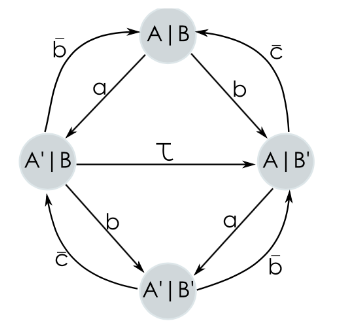
\includegraphics[width=0.3\linewidth]{images/sync-example.png}
    \caption{LTS of $A|B$.}
    \label{fig:sync-example}
\end{figure}

\begin{gather*}
    \frac{\frac{a.A'\xrightarrow{a}A'}{A\xrightarrow{a}A'}A\triangleq a.A'}{A|B\xrightarrow{a}A'|B}\hspace{1cm}\frac{\frac{b.B'\xrightarrow{b}B'}{B\xrightarrow{b}B'}B\triangleq b.B'}{A|B\xrightarrow{b}A|B'}\\
    \frac{
    \frac{\overline{b}.A\xrightarrow{\overline{b}}A}{A'\xrightarrow{\overline{b}}A}
    A'\triangleq\overline{b}.A\hspace{.2cm}
    \frac{b.B'\xrightarrow{b}B'}{B\xrightarrow{b}B'}
    B\triangleq b.B'}
    {A'|B\xrightarrow{\tau}A|B'}
\end{gather*}

When we construct the Labeled Transition System (LTS) for $A|B$, we "lose the consciousness of the parallel". This means the resulting LTS can be described using the standard syntax for non-deterministic processes, even though it was generated from a parallel composition. The parallel operator is valuable because it is the fundamental building block of concurrency theory and allows for a more compact and intuitive representation of complex systems.

Applying the restriction operator to the name $b$ in the system $(A|B)\backslash b$ significantly alters its behavior. The restriction effectively "hides" or deletes any transitions labeled with $b$ or $\overline{b}$ that would otherwise be visible to the outside. However, the $\tau$ action generated by the synchronization on $b$ remains present. This is because the purpose of $\tau$ is specifically to signal that a synchronization has occurred while hiding the underlying event.

\begin{figure}[ht]
    \centering
    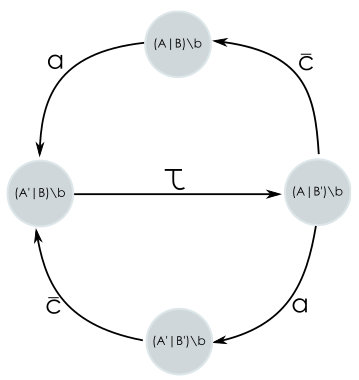
\includegraphics[width=0.3\linewidth]{images/sync-example2.png}
    \caption{LTS of $A|B$ with a restriction on $b$.}
    \label{fig:sync-example2}
\end{figure}

\begin{align*}
    \frac{
    \frac{
    \frac{a.A'\xrightarrow{a}A'}{A\xrightarrow{a}A'}A\triangleq a.A'
    }{A|B\xrightarrow{a}A'|B}}
    {(A|B)\backslash b\xrightarrow{a}(A'|B)\backslash b}a \notin\{b, \overline{b}\}
    \hspace{1cm}
    \frac{
    \frac{
    \frac{b.B'\xrightarrow{b}B'}{B\xrightarrow{b}B'}B\triangleq b.B'
    }{A|B\xrightarrow{b}A|B'}}
    {(A|B)\backslash b\xrightarrow{b}(A|B')\backslash b}b \notin\{b, \overline{b}\}
\end{align*}

In some cases, applying restriction can cause entire states to disappear from the LTS. For example, if we were to restrict both $a$ and $b$ in a system like $(A'|B)\backslash a,b$, any states that are only reachable via those actions would become inaccessible in the restricted system.

\begin{figure}[ht]
    \centering
    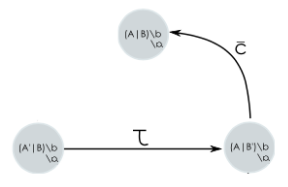
\includegraphics[width=0.4\linewidth]{images/sync-example3.png}
    \caption{LTS of $A'|B$ with a restriction on $a,b$.}
    \label{fig:sync-example3}
\end{figure}

\section{Image Finiteness}
\begin{Thm}{Image Finiteness}{}
    \begin{equation*}
        |\{P':\exists\alpha.P\xrightarrow{a}P'\}|<\infty
    \end{equation*}

\begin{demonstration}
    For every process $P$, let $\mathcal{T}(P)$ be the set of derivation trees for every possible transition $P\xrightarrow{\alpha}P'$, for every $\alpha$ and $P'$. Let us denote with $k_P$ the maximum height of a tree in $\mathcal{T}(P)$. By induction on $k_P$, let us show that $\{P': \exists \alpha.P\xrightarrow{\alpha}P'\}$ is finite.

    \begin{itemize}
        \item Base case ($k_P = 0$): In this case, it must be that $P\triangleq\sum_{i\in I}\alpha_i.P_i$. Then, we have that
        \begin{equation*}
            |\{P':\exists\alpha.P\xrightarrow{\alpha}P'\}| = |\{P_i:i\in I\}\leq |I|<\infty
        \end{equation*}
        \item Inductive step: We have to analyze three cases, according to the outmost operator in $P$.
        \begin{enumerate}
            \item $P\triangleq Q\backslash a$. All inferences for a reduction from $P$ must have as last rule the one dealing with restriction, i.e.:
            \begin{equation*}
                \frac{Q\xrightarrow{\alpha}Q'}{Q\backslash a\xrightarrow{\alpha}Q'\backslash a}\alpha\notin\{a, \overline{a}\}
            \end{equation*}
            for every possible inference starting from process $Q$.

            Since $k_Q < k_P$, we can use the induction hypothesis and obtain that
            \begin{equation*}
                |\{Q':\exists\alpha.Q\xrightarrow{\alpha}Q'\}|<\infty
            \end{equation*}
            the thesis holds by observing that 
            \begin{equation*}
                \{P':\exists\alpha.P\xrightarrow{\alpha}P'\}\subseteq\{Q'\backslash a:\exists\alpha.Q\xrightarrow{\alpha}Q'\}
            \end{equation*}
            \item $P\triangleq A(a_1\ldots a_n)$. In this case, all inferences of $P$ will be of the form
            \begin{equation*}
                \frac{Q\{a_1/x_1\ldots a_n/x_n\}\xrightarrow{\alpha}Q'}{A(a_1\ldots a_n)\xrightarrow{\alpha}Q'}A(x_1\ldots x_n)\triangleq Q
            \end{equation*}
            where the inference threes for $Q\{a_1/x_1\ldots a_n/x_n\}$ have height lower than $k_P$. By indution,
            \begin{equation*}
                |\{R:\exists\alpha.Q\{a_1/x_1\ldots a_n/x_n\}\xrightarrow{\alpha}R\}|<\infty
            \end{equation*}
            The thesis holds by observing that
            \begin{equation*}
                \{P':\exists\alpha.P\xrightarrow{\alpha}P'\}=\{R:\exists\alpha.Q\{a_1/x_1\ldots a_n/x_n\}\xrightarrow{\alpha}R\}
            \end{equation*}
            \item $P\triangleq P_1|P_2$. In this case, notice that:
            \begin{align*}
                \{P':\exists\alpha.P\xrightarrow{\alpha}P'\} = 
                &\{P_1'|P_2:\exists\alpha.P_1\xrightarrow{\alpha}P_1'\}\\
                &\cup\{P_1|P_2':\exists\alpha.P_2\xrightarrow{\alpha}P_2'\}\\
                &\cup\{P_1'|P_2':\exists a.P_1\xrightarrow{a}P_1'\land P_2\xrightarrow{\overline{a}}P_2'\}\\
                &\cup\{P_1'|P_2':\exists a.P_1\xrightarrow{\overline{a}}P_1'\land P_2\xrightarrow{a}P_2'\}
            \end{align*}
            The required cardinality is thus at most the sum of the cardinalates of the four sets depicted above. By induction, we have that every such set has a finite cardinality. The easily allows us to conclude.
        \end{enumerate}
    \end{itemize}
\end{demonstration}
\end{Thm}

\subsection{Renamings}
Finally, CCS includes the concept of \textit{renaming}\index{renaming}. This allows for the transformation of actions within a process according to a mapping function, which is useful for reusing process definitions in different contexts while ensuring they can still synchronize correctly with other components.

Renaming is defined as a function $\sigma:\mathcal{N}\to\mathcal{N}$. By definition, we let $\sigma(\overline{a})$ to be $\overline{\sigma(a)}$ and $\sigma(\tau)$ be $\tau$ itself.

We now define the result of applying a renaming $\sigma$ to a process $P$:
\begin{gather*}
    \sigma(\sum_{i\in I}\alpha_i.P_i) = \sum_{i\in I}\sigma(\alpha_i).\sigma(P_i)\\
    \sigma(P\backslash a) = \sigma(P)\backslash \sigma(a)\\
    \sigma(P_1|P_2) = \sigma(P_1)|\sigma(P_2)\\
    \sigma(A(a_1,\ldots ,a_n)) = A^\sigma(\sigma(a_1),\ldots ,\sigma(a_n))
\end{gather*}
where for every process definition $A(x_1,\ldots ,x_n)\triangleq P$, assume the new process definition
\begin{equation*}
    A^\sigma(\sigma(x_1),\ldots ,\sigma(x_n))\triangleq \sigma(P)
\end{equation*}

\begin{Thm}{If $P\xrightarrow{\alpha}P'$ then $\sigma(P)\xleftrightarrow{\sigma(\alpha)}\sigma(P')$}{}
For every injective $\sigma: \mathcal{N}\to\mathcal{N}$, if $P\xrightarrow{\alpha}P'$ then $\sigma(P)\xrightarrow{\sigma(\alpha)}\sigma(P')$.
\begin{demonstration}
    The proof is by induction the height of the inference for $P\xrightarrow{\alpha}P'$.
    \begin{itemize}
        \item Best case. The only possible such case is with a sum, i.e. $P=\sum_{i \in I}\alpha_i.P_i\xrightarrow{\alpha_j}P_j$.
        In this case, $\alpha =\alpha_j$ and $P'=P_j$, for some $j\in I$.
        We now have that $\sigma(P)=\sum_{i\in I}\sigma(\alpha_i).\sigma(P_i)$ and $\sigma(P)\xrightarrow{\sigma(\alpha_j)}\sigma(P_j)$ $\forall j\in I$.
        \item Inductive step. We have to consider three possible cases:
        \begin{enumerate}
            \item $P\triangleq A(a_1\ldots a_n),A(x_1\ldots x_n)\triangleq Q$ and $Q\{a_1/x_1\ldots a_n/x_n\}\xrightarrow{\alpha}P'$.
            By definition of renaming, we have that $\sigma(P)=A^\sigma(\sigma(a_1)\ldots \sigma(a_n))$.
            By inductive hypothesis on $Q$, we have that
            \begin{equation*}
                \sigma(Q)\{\sigma(a_1)/\sigma(x_1)\ldots \sigma(a_n)/\sigma(x_n)\}\xrightarrow{\sigma(\alpha)}\sigma(P')
            \end{equation*}
            and we conclude.
            \item $P\triangleq Q\backslash a$, $Q\xrightarrow{\alpha}Q'$ and $\alpha\notin\{a,\overline{a}\}$.
            By definition of renaming, $\sigma(Q\backslash a)=\sigma(Q)\backslash \sigma(a)$.
            By induction, $\sigma(Q)\xrightarrow{\sigma(\alpha)}\sigma(Q')$.
            Since $\sigma(\alpha)\notin\{\sigma(a),\overline{\sigma(a)}\}$, we have the desired $\sigma(P)\xrightarrow{\sigma(\alpha)}\sigma(P')$.
            Notice that here injectiveness of $\sigma$ is crucial.
            For example, let $Q=b.0$ and $\sigma(a)=\sigma(b)=a$; then, $P\xrightarrow{b}0\backslash a$ whereas $\sigma(P)\not\xrightarrow{\sigma(b)}0\backslash \sigma(a)$.
            \item $P\triangleq P_1|P_2$.
        \end{enumerate}
    
    \end{itemize}
\end{demonstration}
\end{Thm}

\section{Restrictions}
The interaction between the restriction\index{restriction} operator and process prefixes provides a clear demonstration of how CCS manages the visibility and availability of actions. Consider the proposition stating that
\begin{equation*}
    a.P\backslash a\sim 0
\end{equation*}
This equivalence highlights that restricting a name $a$ effectively "blocks" the process from performing that specific action.

To prove this, we define a relation $S=\{(a.P\backslash a,0)\}$. For this to be a bisimulation, every challenge posed by one process must be met by the other. However, when we examine the challenges possible for $a.P\backslash a$, we find that the process is "stuck." While the inner process $a.P$ is capable of performing the action $a$ to become $P$, the restriction operator $\backslash a$ forbids any transition labeled with $a$. Consequently, $a.P\backslash a$ cannot perform any transitions at all. Since the process $0$ also possesses no transitions, there are no challenges to meet on either side. Thus, the two processes are bisimilar. The same logic applies to the production of an event, where $\overline{a}.P\backslash a\sim 0$, as the restriction operator treats the name and its complement symmetrically.

\subsection{Idempotency of Sum}
A fundamental algebraic property of the choice operator in CCS is idempotency. This is formally expressed by the proposition 
\begin{equation*}
    \alpha.P+\alpha.P+M\sim \alpha.P+M
\end{equation*}
where $M$ represents an arbitrary summation of processes $\sum_{i\in I}\beta_i.P_i$. This property suggests that having multiple identical choices does not change the observable behavior of a system.

The construction of the bisimulation relation for this property requires careful consideration of the states reached after an action is performed. If we initially propose a simple relation $S=\{(\alpha.P+\alpha.P+M,\alpha.P+M)\}$, we encounter a problem during the transition analysis. If the first process performs the action $\alpha$ to become $P$, the second process can also perform $\alpha$ to become $P$. However, for $S$ to be a bisimulation, the pair $(P,P)$ must also be present in the relation. In a general context, $P$ is not necessarily the same as the original sum, so $(P,P)$ is not initially in $S$.

To rectify this, we might expand the relation to $S=\{(\alpha.P+\alpha.P+M,\alpha.P+M)\}\cup\{(P,P)\}$. Yet, even this is insufficient; if $P$ can perform a further action $\beta$ to reach a state $P'$, the pair $(P',P')$ would also need to be included. Therefore, the complete bisimulation relation is defined as $S=\{(\alpha.P+\alpha.P+M,\alpha.P+M)\}\cup Id$, where $Id$ is the identity relation containing all pairs $(Q,Q)$ for any process $Q$. This ensures that once both sides of the equivalence transition into the same process $P$, they can mirror each other's actions indefinitely.\\\\
The utility of bisimulation as a tool for verifying concurrent systems is exemplified by the modeling of n-ary semaphores. An n-ary semaphore $S^{(n)}(p,v)$ is a synchronization primitive that ensures no more than $n$ instances of a specific activity are executing concurrently. The action $p$ starts an activity, while the action $v$ terminates it.

A unary semaphore ($S^{(1)}$) is specified as a process that strictly alternates between $p$ and $v$:
\begin{align*}
    &S^{(1)}\triangleq p.S_1^{(1)}\\
    &S_1^{(1)}\triangleq v.S^{(1)}\\
\end{align*}

A binary semaphore ($S^{(2)}$), which allows up to two concurrent activities, can be defined by its expected state-based behavior. 
\begin{align*}
    &S^{(1)} \triangleq p.S_1^{(2)}\\
    &S_1^{(2)} \triangleq p.S_2^{(2)} + v.S^{(2)}\\
    &S_2^{(2)} \triangleq v.S_1^{(2)}
\end{align*}

To verify a concrete implementation, we can compare this specification against a system composed of two unary semaphores running in parallel: $S^{(1)}|S^{(1)}$.

To prove that the implementation $S^{(1)}|S^{(1)}$ is bisimilar to the specification $S^{(2)}$ ($S^{(1)}|S^{(1)}\sim S^{(2)}$), we construct a bisimulation relation $S$ that maps the collective states of the two parallel processes to the corresponding states of the binary semaphore:
\begin{equation*}
    S=\{(S^{(1)}|S^{(1)},S^{(2)}),(S_1^{(1)}|S^{(1)},S_1^{(2)}),(S^{(1)}|S_1^{(1)},S_1^{(2)}), (S_1^{(1)}|S_1^{(1)},S_2^{(2)})\}
\end{equation*}

In this relation:
\begin{itemize}
    \item The initial state $S^{(1)}|S^{(1)}$ corresponds to the binary semaphore with zero active processes.
    \item The state $S_1^{(1)}|S^{(1)}$ represents the situation where one of the two semaphores has performed a $p$ action, corresponding to the binary semaphore having one active process.
    \item The state $S_1^{(1)}|S_1^{(1)}$ represents both semaphores having performed $p$, meaning the capacity of the binary semaphore (two active processes) is reached.
\end{itemize}

Showing that this relation is a bisimulation confirms that the modular implementation of two single-capacity semaphores behaves exactly like one double-capacity semaphore.

\subsection{Congruence}
The ultimate goal of defining process equivalences like bisimulation is to enable "equational reasoning." This allows designers to replace a component $P$ with an equivalent component $Q$ within a larger system without altering the system's overall behavior. An equivalence that supports this substitutability is known as a \textit{congruence}\index{congruence}.

To define congruence formally, we introduce the concept of an execution context $C$. A context is essentially a process with a "hole" (denoted by $\square$). When we place a process $P$ into this hole, we denote the resulting system as $C[P]$. For example, if we have a context $C=(\square|Q)\backslash a$, then $C[P]$ results in the process $(P|Q)\backslash a$.

The set $\mathcal{C}$ of CCS contexts is given by the following grammar:
\begin{equation*}
    C ::= \square|C \scalebox{0.8}{$|$} P | C\backslash a | \alpha.C+M
\end{equation*}
where $M$ denotes a sum.

An equivalence relation $\mathcal{R}$ is a congruence if and only if
\begin{equation*}
    \forall(P, Q)\in \mathcal{R}, \forall C.(C[P], C[Q])\in \mathcal{R}
\end{equation*}

An equivalence $\sim$ is a congruence if, for any two processes $P$ and $Q$ such that $P\sim Q$, it is also the case that $C[P]\sim C[Q]$ for every possible context $C$. While not all behavioral equivalences are congruences, strong bisimulation in CCS is a congruence for most operators, allowing for the modular verification and simplification of complex concurrent systems.

\begin{Lemma}{If $P\sim Q$ then $\alpha.P+M\sim \alpha.Q+M$.}{}
If $P\sim Q$ then $\alpha.P+M\sim \alpha.Q+M$, for all $\alpha$ and $M$.

\begin{demonstration}
    It is sufficient to show that
    \begin{equation*}
        S=\{(\alpha.P+M, \alpha.Q+M): P\sim Q, \alpha \in A, M=\sum_{i\in I}\alpha_i.P_i\}\cup \sim
    \end{equation*}
    is a simulation.

    Let $(\alpha.P+M, \alpha.Q+M)\in S\hspace{.5cm}\alpha.P+M\xrightarrow{\beta}P'\hspace{.5cm}M=\sum_{i \in I}\alpha_i.P_i$.
    \begin{enumerate}
        \item $\beta = \alpha$ and $P' = P$. $\alpha.Q+M$ can reply with actions $\alpha$ and become $Q$ by hypothesis, is bisimilar to $P$.
        \item $\beta = \alpha_j$, for some $j\in I$, and $P' = P_j$. $\alpha.Q + M$ can reply with the same action and by reducing to the same process.
    \end{enumerate}
\end{demonstration}
\end{Lemma}

\begin{Lemma}{If $P\sim Q$ then $P\backslash a\sim Q\backslash a$}{}
    If $P\sim Q$ then $P\backslash a\sim Q\backslash a$, for all $a$.
\begin{demonstration}
    Also in this case, let us show that
    \begin{equation*}
        S = \{(P\backslash a, Q\backslash a):\forall P\sim Q, \forall a\in \mathcal{N}\}
    \end{equation*}
    is a simulation.
    
    Let $(P\backslash a, Q\backslash a)\in S$ and $P\backslash a\xrightarrow{\alpha}P'$. $P' = P''\backslash a$, for $P\xrightarrow{\alpha}P''$ and $\alpha\notin\{a, \overline{a}\}$.

    Process $Q$ can perform the same action $\alpha$ and reduce to process $Q'=Q''\backslash a$. Since $P\sim Q$, we have that $P''\sim Q''$.
\end{demonstration}
\end{Lemma}

\begin{Lemma}{If $P\sim Q$ then $P|R\sim Q|R$}{}\label{lemma:pq-pbarrqbarr}
If $P\sim Q$ then $P|R\sim Q|R$, for all $R$.
\begin{demonstration}
    Let us show that
    \begin{equation*}
        S = \{(P|R, Q|R): P\sim Q\}
    \end{equation*}
    is a simulation. Let $(P|R, Q|R)\in S$ and $P|R\xrightarrow{\alpha}P'$.
    \begin{enumerate}
        \item $P\xrightarrow{\alpha}P''$ and $P' = P''|R$. Since $P\sim Q$, we have that $Q\xrightarrow{\alpha}Q''$ and $P''\sim Q''$; hence, $Q|R\xrightarrow{\alpha}Q''|R$ and $(P''|R, Q''|R)\in S$.
        \item $R\xrightarrow{\alpha}R'$ and $P' = P|R$. Trivially, $Q|R\xrightarrow{\alpha}Q|R'$ and $(P|R', Q|R')\in S$.
        \item $P\xrightarrow{\alpha}P''\land R\xrightarrow{\overline{a}}R''$ (or viceversa) and $P'=P''|R''$, with $\alpha = \tau$. Since $P\sim Q$, we have that $Q\xrightarrow{a}Q''$ and $Q''\sim P''$. Hence, $Q|R\xrightarrow{\tau}Q''|R''=Q'$ and $(P', Q')\in S$.
    \end{enumerate}
\end{demonstration}
\end{Lemma}

\begin{Thm}{If $P\sim Q$ then $\forall C.C[P]\sim C[Q]$.}{}
If $P\sim Q$ then $\forall C.C[P]\sim C[Q]$.
\begin{demonstration}
    By induction on the structure of $C$.
    \begin{itemize}
        \item Base case. The only possible context to analyze is $C=\square$. 
        
        We have that $C[P]=P$, for all $P$. Hence, $C[P]\sim C[Q]$ by hypothesis.
        \item Inductive step. Let us reason on the possible structure of $C$ and exploit the previous lemmata.

        For example, if $C = R|C'$, for some other context $C'$, then $C[P]=R|C'[P]$ and $C[Q]=R|C'[Q]$. 
        
        By induction (since $C'$ is smaller then $C$), we have that $C'[P]\sim C'[Q]$, by the previous Lemmata, we obtain that $R|C'[P]\sim R|C'[Q]$.
    \end{itemize}
\end{demonstration}
\end{Thm}

\chapter{Weak Bisimilarity}
The notion of equivalence studied in previous chapters, often referred to as strong bisimulation, is highly discriminating. For instance, it distinguishes between the processes $\tau.P$ and $\tau.\tau.P$. Such a distinction is logical only if an external observer has the capacity to count individual non-observable actions (the $\tau$ transitions). However, if we operate under the assumption that an observer cannot access the internal information or silent steps of a system, this level of discrimination becomes unacceptable. To address this, we introduce the concept of \textit{weak bisimilarity}\index{weak bisimilarity}, which equates processes based strictly on their observable behavior—their visible actions—while ignoring the internal structure and internal transitions that do not affect the environment.

The fundamental principle behind weak bisimilarity is the abstraction of internal $\tau$ actions. This abstraction requires a revised understanding of how processes "reply" to one another's transitions:
\begin{itemize}
    \item A visible action must be replied to with the same visible action, though it may be preceded or followed by any number of internal $\tau$ actions.
    \item An internal action must be replied to by a sequence of internal actions, which may potentially be empty.
\end{itemize}

To formalize this, we define an extended transition relation $\Rightarrow$. We say $P\Rightarrow P'$ if $P$ can reach $P'$ through zero or more silent transitions. Building on this, the relation $\xRightarrow{\widehat{\alpha}}$ is defined such that if $\alpha=\tau$, then $\xRightarrow{\widehat{\tau}}$ is simply $\Rightarrow$ (zero or more $\tau$ steps); if $\alpha$ is a visible action, then $\xRightarrow{\widehat{\alpha}}$ represents the sequence $\Rightarrow\xrightarrow{\alpha}\Rightarrow$.

Weak bisimulation is defined analogously to strong bisimulation, but it utilizes these extended transitions. Specifically, if $(p,q)\in S$, then for every $p\xrightarrow{\alpha}p'$, there must exist a $q\xrightarrow{\widehat{\alpha}}q'$ such that $(p',q')\in S$. We say $p\approx q$ (weakly bisimilar) if such a relation exists. It is important to note that every strong bisimulation is also a weak bisimulation, meaning that strongly bisimilar processes are always weakly bisimilar, though the inverse is not necessarily true.

\begin{Definition}{Weak Bisimulation}{}
    $S$ is a weak simulation if and only if $\forall (p, q)\in S$ $\forall p\xrightarrow{\alpha}p'$ $\exists q'$ s.t. $q\xRightarrow{\widehat{\alpha}}q'$ and $(p', q')\in S$.

    A relation $S$ is called weak bisimulation if both $S$ and $S^{-1}$ are weak simulations.

    We say that $p$ and $q$ are weakly bisimilar, written $p\approx q$, if there exists a weak bisimulation $S$ such that $(p, q)\in S$.
\end{Definition}

\begin{figure}[ht]
    \centering
    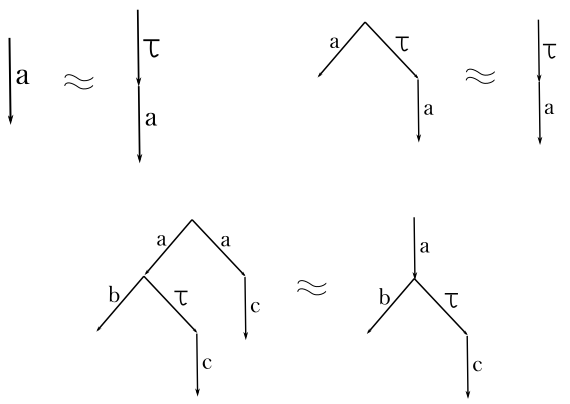
\includegraphics[width=0.6\linewidth]{images/weak-bisim-example.png}
    \caption{Example of Weak Bisimilar Processes.}
    \label{fig:weak-bisim-example}
\end{figure}

\begin{Thm}{Weak Bisimilarity}{}
    Given any process $P$ and any sum $M, N$, then:
    \begin{enumerate}
        \item $P\approx\tau.P$;
        \item $M+N+\tau.N\approx M+\tau.N$;
        \item $M+\alpha.P+\alpha.(N+\tau.P)\approx M+\alpha.(N+\tau.P)$.
    \end{enumerate}

    \begin{demonstration}
        Take a simmetric closure of the following relations, that can be easly shown to be weak simulations:
        \begin{enumerate}
            \item $S=\{(P, \tau.P)\}\cup Id$
            \item $S=\{(M+N+\tau.N,M+\tau.N)\}\cup Id$
            \item $S=\{(M+\alpha.P+\alpha.(N+\tau.P), M+\alpha.(N+\tau.P))\}\cup Id$
        \end{enumerate}
    \end{demonstration}
\end{Thm}

While weak bisimilarity is less sensitive to transitions than strong bisimilarity, it does not mean internal actions can be ignored entirely. Internal actions can still lead to observable differences in behavior, particularly regarding nondeterministic choices.

\begin{figure}[ht]
    \centering
    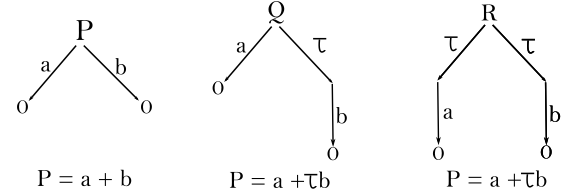
\includegraphics[width=0.6\linewidth]{images/weak-bisim-pqr.png}
    \caption{Weack Bisimilarity abstracts from any $\tau$?}
    \label{fig:weak-bisim-pqr}
\end{figure}

Consider the processes $P,Q$, and $R$ illustrated in Figure \ref{fig:weak-bisim-pqr}:

The process $P$ is defined as $a+b$. Process $Q$ is defined as $a+\tau.b$. Despite the presence of the internal action, $P$ and $Q$ are not weakly bisimilar.

To see why, suppose a weak bisimulation $S$ exists that contains $(P,Q)$. Process $Q$ can perform an internal transition $Q\xrightarrow{\tau}b.0$. According to the definition of weak simulation, $P$ must be able to match this with a transition $P\Rightarrow P'$ such that $(P',b.0)\in S$. Since $P$ has no $\tau$ transitions, the only state $P$ can reach via zero or more $\tau$ steps is $P$ itself ($P\Rightarrow P$). However, $(P,b.0)$ cannot be in the bisimulation because $P$ can perform an a action, whereas $b.0$ cannot. This contradiction proves that $P\not\approx Q$. In a similar fashion, it can be shown that $P,Q$, and $R$ are all pairwise non-bisimilar.

\section{Example: Factory}
A factory activity is specified to handle three types of work: easy ($E$), medium ($M$), and difficult ($D$). The activity $A$ receives an input ($i_E$,$i_M$, or $i_D$) and produces a manufactured output $\overline{o}$.
\begin{align*}
    &A\triangleq i_E.A'+i_M.A'+i_D.A'\\
    &A'\triangleq \overline{o}.A
\end{align*}

The total factory specification is the parallel composition of two such activities: 
\begin{equation*}
Factory\triangleq A|A.
\end{equation*}

The implementation involves two workers ($W$) and two shared machines: a general machine ($G$) and a special machine ($S$). Workers share these machines via semaphores.
\begin{itemize}
    \item \textit{Easy works:} Handled by the worker without machinery.
    \item \textit{Medium works:} The worker can use either the general or the special machine.
    \item \textit{Difficult works:} The worker must use the special machine.
\end{itemize}
    
The worker $W$ is defined by its ability to accept input and transition into states $W_E$,$W_M$, or $W_D$. If machines are required, the worker performs internal synchronization actions: $rg$,$rs$ to request a machine, and $lg$,$ls$ to leave it. 

\begin{align*}
    W&\triangleq i_E.W_E+i_M.W_M+i_D.W_D \hspace{1.1cm}S\triangleq rs.S'\\
    W_E&\triangleq \overline{o}.W \hspace{4.35cm}S'\triangleq ls.S\\
    W_M&\triangleq\overline{rg}.\overline{lg}.W_E+\overline{rs}.\overline{ls}.W_E \hspace{1.95cm}G\triangleq rg.G'\\
    W_D&\triangleq \overline{rs}.\overline{ls}.W_E \hspace{3.7cm}G'\triangleq lg.G
\end{align*}

The implementation of the system is:
\begin{equation*}
    Workers\triangleq (W|W|G|S)\backslash_{\{rg,rs,lg,ls\}}
\end{equation*}

To prove that the implementation is correct, we show that $Factory\approx Workers$. This is done by exhibiting a weak bisimulation relation $R$ that contains the pair $(A|A,Workers)$.

The relation $R$ is quite large because it must account for all possible combinations of workers being in different states of their tasks. It is a family of relations including:
\begin{itemize}
    \item Pairs where both activities are idle.
    \item Pairs where one worker has accepted work $x$ and the other is idle.
    \item Pairs where workers are in the process of leaving machines ($lg.W_E$ or $ls.W_E$).
    \item Pairs where both workers are active with different work types $x$ and $y$.
\end{itemize}

Here we provide a shorter form:
\begin{align*}
    R = \{
        &(A|A, (W|W|G|S)\backslash_N), (A|A', (W|W_x|G|S)\backslash_N),\\
        &(A|A', (W|\overline{lg}\cdot W_E|G'|S)\backslash_N), (A|A', (W|\overline{ls}\cdot W_E|G|S')\backslash_N),\\
        &(A'|A', (W_y|W_x|G|S)\backslash_N), (A'|A', (W_y|\overline{lg}\cdot W_E|G'|S)\backslash_N),\\
        &(A'|A', (W_y|\overline{ls}\cdot W_E|G|S')\backslash_N), (A'|A', (\overline{lg}\cdot W_E|\overline{ls}\cdot W_E|G'|S')\backslash_N)
    \}
\end{align*}

In total, accounting for the different work types ($E,M,D$) and the commutativity of the parallel operator, the relation $R$ consists of 34 distinct pairs. While these proofs can become cumbersome by hand, they demonstrate that the Workers system effectively replicates the visible behavior of the Factory specification while hiding the internal details of machine acquisition and release.

\section{Example: Lottery}
In modeling a lottery system, denoted as $L$, we consider a scenario where a ball is nondeterministically selected from a bag containing $n$ balls. Once an extraction occurs, the ball is replaced in the bag, allowing the procedure to repeat indefinitely. The formal specification for this behavior is defined as:
\begin{equation*}
    L\triangleq \tau.\overline{p_1}.L+\tau.\overline{p_2}.L+\ldots+\tau.\overline{p_n}.L    
\end{equation*}

In this expression, the internal $\tau$ actions represent the extraction of a ball, which is not directly observable by an external user. The observable action $\overline{p_i}$ represents the communication of the value of the $i$-th extracted ball to the environment (see Figure \ref{fig:lottery}).

\begin{figure}[ht]
    \centering
    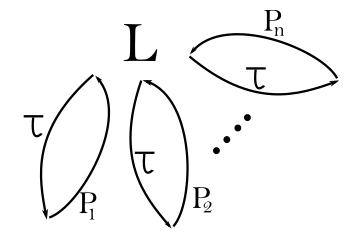
\includegraphics[width=0.35\linewidth]{images/lottery.png}
    \caption{Lottery LTS.}
    \label{fig:lottery}
\end{figure}

To implement this specification, we can construct a system comprising $n$ distinct components, with each component representing one ball in the lottery. Each ball component moves through three distinct states to manage the extraction process:
\begin{itemize}
    \item \textit{State A:} The component is waiting to be "habilitated" for extraction, meaning it does not yet have the authority to be picked.
    \item \textit{State B:} The component is now habilitated. In this state, a nondeterministic choice occurs: the ball can either be extracted (leading to state $C$) or it can pass the habilitation "token" to the next ball in the sequence, returning itself to state $A$.
    \item \textit{State C:} The ball has been extracted and is waiting to communicate its value $\overline{p_i}$ externally before returning to a state where it can eventually be habilitated again.
\end{itemize}

\begin{align*}
    &A_i = a_i.B_i\\
    &B_i = \tau.C_i+\overline{a}_{(i \mod n)+1}.A_i\\
    &C_i = \overline{p_i}.B_i
\end{align*}

This implementation relies on a token ring mechanism where actions $a_i$ represent the passing of a token among the balls. Only the ball currently holding the token has the capacity to be extracted. The token is initially assigned to the first ball, $B_1$, though this choice of starting position is immaterial to the system's overall behavior. The full implementation is defined by the parallel composition of these components, with the internal token-passing actions restricted (see Figure \ref{fig:lottery-impl}):

\begin{equation*}
    Impl\triangleq (B_1|A_2|\ldots|A_n)\backslash_{\{a_1,\ldots,a_n\}}
\end{equation*}

\begin{figure}[ht]
    \centering
    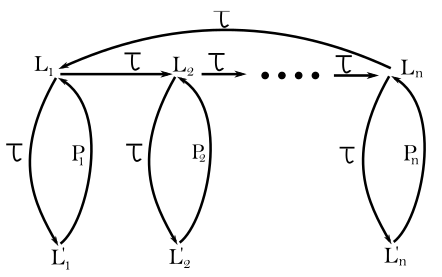
\includegraphics[width=0.5\linewidth]{images/lottery-impl.png}
    \caption{Lottery Implementation LTS.}
    \label{fig:lottery-impl}
\end{figure}

where
\begin{align*}
    L_i &= (A_1|\ldots|A_{i-1}|B_i|A_{i+1}|\ldots|A_n)\backslash_{\{a_1,\ldots,a_n\}}\\
    L_i' &= (A_1|\ldots|A_{i-1}|C_i|A_{i+1}|\ldots|A_n)\backslash_{\{a_1,\ldots,a_n\}}
\end{align*}

We now want to show that this system implementation is correct with respect to the given specification:
\begin{equation*}
    L\approx Impl
\end{equation*}

We shall prove a more general result, i.e. that, for every $i= 1,\ldots,n$, we have that 
\begin{equation*}
    L\approx L_i
\end{equation*}

Since $Impl = L_i$, this suffices to conclude.

Through the lens of weak bisimilarity, this decentralized token-passing system is equivalent to the centralized specification $L$ because the internal token movements and extraction choices are hidden from the observer.

We prove that 
\begin{equation*}
    \mathcal{R}\triangleq \{(L, L_i) | 0<i\leq n\} \cup \{(\overline{p_i}.L, L'_i) | 0<i\leq n\}
\end{equation*}
and $\mathcal{R}^{-1}$ are weak simulations.

\section{Example: Scheduler}
A more complex application of these principles is the design of a scheduler for a set of $n$ processes, $P_i$. The scheduler's primary responsibility is to ensure that these processes start their tasks cyclically, beginning with $P_1$. While the executions of different processes are permitted to overlap, the scheduler must enforce a strict constraint: each specific process $P_i$ must complete its current task before it can be started again.

In this model, a process $P_i$ requests to start via action $a_i$ and signals termination via action $b_i$. Therefore, the scheduler must guarantee that all $a_i$ actions occur in a cyclic sequence ($a_1,a_2,\ldots,a_n,a_1,\ldots$) and that for every individual $i$, the start action $a_i$ alternates with the termination action $b_i$. The specification state $S_{i,X}$ represents a system waiting for the activation of process $P_i$, where $X$ is the set of indices of processes that are currently active. The initial configuration is $S_{i,\empty}$.

\begin{equation*}
    S_{i,X}=\begin{cases}
        \sum_{j\in X}b_j.S_{i,X-\{j\}} & \textit{if }i \in X\\
        a_i.S_{(i\mod n)+1,X\cup\{i\}}+\sum_{j\in X}b_j.S_{i,X-\{j\}} &\textit{otherwise}
    \end{cases}
\end{equation*}

\begin{figure}[ht]
    \centering
    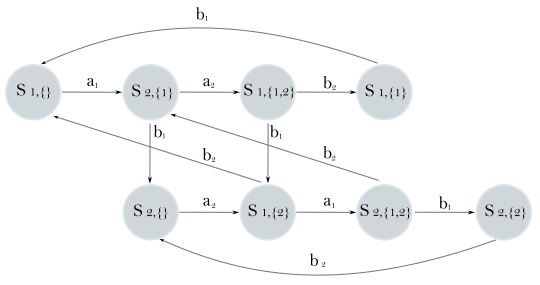
\includegraphics[width=0.7\linewidth]{images/sched-n2.png}
    \caption{Scheduler LTS for $n = 2$.}
    \label{fig:sched-n2}
\end{figure}

One might attempt to implement this scheduler using a token ring similar to the lottery example. In this proposed implementation, we define four states for each component:
\begin{itemize}
    \item $A_i=a_i.B_i$ (waiting for start action $a_i$)
    \item $B_i=\overline{c}_{(i \mod n)+1}.C_i$ (signaling the next process that it may start)
    \item $C_i=b_i.D_i$ (waiting for process termination $b_i$)
    \item $D_i=c_i.A_i$ (receiving the signal to eventually start again)
\end{itemize}

\begin{figure}[ht]
    \centering
    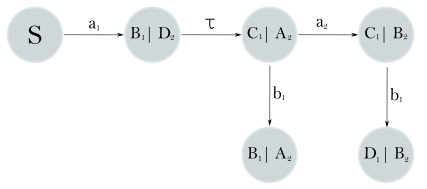
\includegraphics[width=0.55\linewidth]{images/sched-restr.png}
    \caption{Scheduler LTS where in every state, names $c_1$ and $c_2$ are restricted.}
    \label{fig:sched-restr}
\end{figure}

The system is $S=(A_1|D_2|\ldots |D_n)\backslash_{\{c_1,\ldots,c_n\}}$. However, testing for weak bisimilarity ($S\approx S1,\emptyset$) reveals that this implementation is incorrect. By examining the Labelled Transition System (LTS) for the case where $n=2$ (Figure \ref{fig:sched-n2}), a discrepancy arises: in the specification, the state $S_{1,\{1,2\}}$ (where both processes are active) can perform the action $b_2$. In the implementation state $(C_1|B_2)_{\backslash\{c_1,c_2\}}$ (Figure \ref{fig:sched-restr}), the action $b_2$ is not immediately available.

The root of this error is an unintended constraint added during implementation: process $i$ is forced to pass the token ($\overline{c}_i+1$) before it can perform its termination action $b_i$. In the specification, the termination of one process is not strictly ordered relative to the start or end of others, provided the cyclic and alternating rules are met. To fix this, the state $C_i$ must be redefined to allow the process to either terminate or receive a token in any order:
\begin{equation*}
    C_i=b_i.D_i+c_i.b_i.A_i    
\end{equation*}

This corrected implementation removes the erroneous dependency, ensuring the implementation is weakly bisimilar to the original specification.

\chapter{Inference Systems for Bisimilarity}
In the study of concurrent systems, establishing whether two processes exhibit the same behavior is a fundamental challenge. While we have previously explored bisimilarity through transitions and relations, we can also approach the problem using an \textit{inference system}\index{inference system}. This method allows us to determine if two processes are bisimilar by starting from a collection of established axioms and applying specific inference rules.  

For the scope of this discussion, we restrict our focus to finite processes, which are those constructed without recursive process definitions. Although a limited handling of recursion is possible, it is important to note that deciding bisimilarity for general, unrestricted processes is actually an undecidable problem.

The effectiveness of such an inference system is measured by two key properties:
\begin{itemize}
    \item \textit{Soundness:}\index{soundness} This ensures that any equality we infer using the system is correct, meaning the processes are truly bisimilar.  
    \item \textit{Completeness:}\index{completeness} This ensures that if two processes are indeed bisimilar, the system is powerful enough to allow us to infer their equality.
\end{itemize}

\section{Axioms and Rules for Strong Bisimilarity}
The inference system for strong bisimilarity is built upon several groups of axioms that define the fundamental nature of process operators.  

\subsection{Axioms for Sum}
\begin{itemize}
    \item Identity
    \begin{equation*}
        \vdash M+0=M
    \end{equation*}
    a process with no moves acts as an identity for choice.  
    \item Commutativity
    \begin{equation*}
        \vdash M_1+M_2=M_2+M_1
    \end{equation*}
    the order of choices does not matter.  
    \item Associativity
    \begin{equation*}
        \vdash M_1+(M_2+M_3)=(M_1+M_2)+M_3    
    \end{equation*}
    allowing us to group choices as needed.  
    \item Idempotency
    \begin{equation*}
        \vdash M+M=M
    \end{equation*}
    offering the same choice twice is the same as offering it once.
\end{itemize}

\subsection{Axiom for Parallel Composition}
The parallel operator uses an expansion law to transform parallel processes into a summation of possible actions. This axiom captures how two processes can either act independently or synchronize:
\begin{align*}
    \vdash \sum_{i}\alpha_i.Pi|\sum_{j}\beta_j.Q_j=&\sum_{i}\alpha_i(P_i|\sum_{j}\beta_j.Q_j)+\\
    &\sum_{j}\beta_j(\sum_{i}\alpha_i.P_i|Q_j)+\\
    &\sum_{\alpha_i=\overline{\beta_j}}\tau (P_i|Q_j)
\end{align*}

Essentially, the result is a sum of all possible prefixes from both sides, plus a $\tau$ action for every possible synchronization between complementary actions $\alpha_i$ and $\overline{\beta_j}$.

\subsection{Axioms for Restriction}
Restriction helps encapsulate internal actions:
\begin{itemize}
    \item Restricting an empty process remains an empty process: 
    \begin{equation*}
        \vdash 0\backslash a=0
    \end{equation*}
    \item The restriction operator distributes over sums: 
    \begin{equation*}
        \vdash(\sum_i\alpha_i.P_i)\backslash a=\sum_i(\alpha_i.P_i)\backslash a
    \end{equation*}
    \item When applied to a prefixed process $\alpha.P$, the action is either removed (becoming 0) if it is the restricted label $a$ or its complement $a$, or it remains if the label is different.
    \begin{equation*}
        \vdash (\alpha.P)\backslash a = \begin{cases}
            0 & \textit{if }\alpha\in\{a, \overline{a}\}\\
            \alpha.(P\backslash a) &\textit{otherwise}
        \end{cases}
    \end{equation*}
\end{itemize}

\subsection{General Inference Rules}
To manipulate these axioms, we use standard equivalence and congruence rules:
\begin{itemize}
    \item Reflexivity, Symmetry, and Transitivity: These establish that = is an equivalence relation (e.g., if $P=Q$ and $Q=R$, then $P=R$):
    \begin{equation*}
        \vdash P = P\hspace{1cm}
        \frac{\vdash P = Q}{\vdash Q = P}\hspace{1cm}
        \frac{\vdash P = Q\hspace{.2cm}\vdash Q = R}{\vdash P = R}
    \end{equation*}
    \item Congruence (Context Closure): If $P=Q$, then for any context $C[\cdot]$, $C[P]=C[Q]$. This allows us to replace bisimilar processes within larger systems:
    \begin{equation*}
        \frac{\vdash P = Q}{\vdash C[P] = C[Q]}
    \end{equation*}
\end{itemize}

\section{Soundness, Completeness, and Standard Forms}
The relationship between provability in this system ($\vdash P=Q$) and strong bisimilarity ($P\sim Q$) is formalized in the following theorem, which states that for finite processes, $P\sim Q$ if and only if $\vdash P=Q$.

\begin{Thm}{Soundness}{}
    If $\vdash P = Q$ then $P\sim Q$.
    \begin{demonstration}\phantom{}
    \begin{itemize}
        \item for every axiom $\vdash LHS = RHS$, let us consider the relation $\{(LHS, RHS)\} \cup Id$ and prove that it is a bisimulation;
        \item the inference rules hold for bisimilarity, since it is an equivalence and a congruence.
    \end{itemize}
    \end{demonstration}
\end{Thm}

\begin{Definition}{Standard form}{}
    $P$ is in \textit{standard form}\index{standard form} if and only if $P\triangleq \sum_i\alpha_i.P_i$ and $\forall_iP_i$ is in standard form.
\end{Definition}

\begin{Lemma}{Standard form}{}
    $\forall P \exists P'$ in standard form such that $\vdash P = P'$.
    \begin{demonstration}
    By induction on the structure of $P$.
    \begin{itemize}
        \item Base case: ($P \triangleq 0$). It suffices to consider $P'\triangleq 0$ and conclude by reflexivity.
        \item Inductive step: We have to consider three cases.
        \begin{enumerate}
            \item $P \triangleq \sum_{i\in I}\alpha_i.P_i$. By induction, we have that $\forall P_i \exists P_i'$ in standard form such that $\vdash P_i = P_i'$. 
            
            From $\vdash P_1 = P_1'$, by context closure w.r.t. context $\alpha.\square+\sum_{i\in I\backslash\{1\}}\alpha_i.P_i$, we have that
            \begin{equation*}
                \vdash \alpha_1.P_1 + \sum_{i\in I\backslash\{1\}}\alpha_i.P_i = \alpha_1.P_1' + \sum_{i\in I\backslash\{1\}}\alpha_i.P_i
            \end{equation*}
            
            From $\vdash P_2 = P_2'$, by context closure w.r.t. context $\alpha_2.\square+(\alpha_1.P_1'+\sum_{i\in I\backslash\{1, 2\}}\alpha_i.P_i)$, we have that
            \begin{equation*}
                \vdash \alpha_2.P_2 + (\alpha_1.P_1' + \sum_{i\in I\backslash\{1, 2\}}\alpha_i.P_i) = \alpha_2.P_2' + (\alpha_1.P_1' + \sum_{i\in I\backslash\{1, 2\}}\alpha_i.P_i)
            \end{equation*}
            
            By transitivity and commutativity of choices, we have that
            \begin{equation*}
                \vdash \sum_{i\in I}\alpha_i.P_i = \sum_{i\in \{1, 2\}}\alpha_i.P_i' + \sum_{i\in I\backslash\{\, 2\}}\alpha_i.P_i
            \end{equation*}

            From $\vdash P_3 = P_3'$, by context closure w.r.t. context $\alpha_3.\square+(\sum_{i\in\{1, 2\}}\alpha_i.P_i'+\sum_{i\in I\backslash\{1, 2, 3\}}\alpha_i.P_i$, we have that
            \begin{equation*}
                \vdash \alpha_3.P_3 + (\sum_{i\in \{1, 2\}}\alpha_i.P_i' + \sum_{i\in I\backslash\{1, 2, 3\}}\alpha_i.P_i) = 
                \alpha_3.P_3'+(\sum_{i\in \{1, 2\}}\alpha_i.P_i'+\sum_{i\in I\backslash\{1, 2, 3\}}\alpha_i.P_i)
            \end{equation*}
            and
            \begin{equation*}
                \vdash \sum_{i\in I}\alpha_i.P_i = \sum_{i \in \{1, 2, 3\}}\alpha_i.P_i' + \sum_{i \in I\backslash\{1, 2, 3\}}\alpha_i.P_i
            \end{equation*}

            We can repeat this reasoning until we obtain
            \begin{equation*}
                \vdash \sum_{i \in I}\alpha_i.P_i = \sum_{i \in I}\alpha_i.P_i'
            \end{equation*}

            \item $P\triangleq P_1 | P_2$ . By induction, we have that $\exists P_1', P_2'$ in standard form such that $\vdash P_1 = P_1'$ and $\vdash P_2 = P_2'$, where $P_1'=\sum_i\alpha_i.R_i$ and $P_2'=\sum_j\beta_j.Q_j$.
            
            From these facts, by context closure, it follows that $\vdash P_1|P_2 = P_1'|P_2$ and $\vdash P_1' | P_2 = P_1'|P_2'$; hence, by transitivity:
            \begin{align*}
                \vdash P_1 | P_2 &= \sum_i\alpha_i.R_i|\sum_j\beta_j.Q_j\\
                &= \sum_i\alpha_i(R_i|\sum_j\beta_j.Q_j) + \sum_j\beta(\sum_i\alpha_i.R_i|Q_j) + \sum_{\alpha_i = \overline{\beta_j}}\tau (R_i|Q_j)\\
                &=\ldots\\
                &=P'
            \end{align*}
            where the elimination of the parallel from standard forms is repeated until there are no more occurrences of $'|'$ in the process.
            \item $P \triangleq Q\backslash a$. By induction, we have that $\exists Q'$ in standard form such that $\vdash Q = Q'$, where $Q' = \sum_{i \in I}\alpha_i.R_i$. From this and by congruence, it follows that
            \begin{align*}
                \vdash Q\backslash a &= Q'\backslash a\\
                &=\sum_{i \in I}(\alpha_i.R_i)\backslash a\\
                &=\sum_{i \in I}\alpha_i(R_i\backslash a)
            \end{align*}
            where $I' = \{i \in I : \alpha_i \notin \{a, \overline{a}\}\}$ and the elimination of restriction is repeated until such an operator is totally removed from the process.
        \end{enumerate}
    \end{itemize}
    \end{demonstration}
\end{Lemma}

\begin{Thm}{Completeness}{}
    If $P\sim Q$ then $\vdash P = Q$.
    \begin{demonstration}
        Because of the previous Lemma, we have that $\exists P', Q'$ in standard form such that $\vdash Q = Q'$ and $\vdash P = P'$, where
        \begin{equation*}
            P'\triangleq \sum_{i = 1}^n\alpha_i.P_i
            \hspace{.5cm}\textit{and}\hspace{.5cm}
            Q'\triangleq \sum_{j = 1}^m\beta_j.Q_j
        \end{equation*}
        We only have to prove that $\vdash P' = Q'$ and, by transitivity, we would obtain $\vdash P = Q$. This proof is done by induction over the maximum height of the syntactic tree that describes $P'$ and $Q'$, i.e. over $max\{h(P'), h(Q')\}$.
        \begin{itemize}
            \item Base case ($0$): in this case, $P' = Q' = 0$ and we trivially conclude.
            \item Induction:
            \begin{align*}
                P'\xrightarrow{\alpha_1}P_1 
                &\Rightarrow P\xrightarrow{\alpha_1}\widehat{P}\textit{ s.t. }P_1\sim \widehat{P}\\
                &\Rightarrow Q\xrightarrow{\alpha_1}\widehat{Q}\textit{ s.t. }\widehat{P}\sim \widehat{Q}\\
                &\Rightarrow Q'\xrightarrow{\alpha_1}Q''\textit{ s.t. }\widehat{Q}\sim Q''
            \end{align*}
            by definition of $Q'$, it must be that $\alpha_1 = \beta_{j_1}$ and $Q'' = Q_{j_1}$ , for some $j_1$.
            
            By transitivity, we obtain that $P_1\sim Q_{j_1}$; hence, by induction, it follows that $\vdash P_1 = Q_{j_1}$.
        \end{itemize}

        Let us now consider the context
        \begin{equation*}
            C\triangleq \alpha_1[]+\sum_{i = 2}^n\alpha_i.P_i
        \end{equation*}
        Then
        \begin{equation*}
            \vdash \alpha_1.P_1 + \sum_{i = 2}^n\alpha_i.P_i = \beta_{j_1}.Q_{j_1} + \sum_{i = 2}^n\alpha_i.P_i
        \end{equation*}
        By iterating this reasoning on every summand of $P'$, we can conclude that
        \begin{align*}
            \vdash P' &= \beta_{j_1}.Q_{j_1} + \sum_{i = 2}^n\alpha_i.P_i\\
            &= \beta_{j_1} + \beta_{j_2}.Q_{j_2} + \sum_{i = 3}^n\alpha_i.P_i\\
            &= \beta_{j_1} + \beta_{j_2}.Q_{j_2} + \beta_{j_3}.Q_{j_3} + \sum_{i = 4}^n\alpha_i.P_i\\
            &= \ldots\\
            &= \sum_{i = i}^n\beta_{j_i}.Q_{j_i}
        \end{align*}
        Similarly, we can prove that
        \begin{equation*}
            \vdash Q' = \sum_{j = 1}^m\alpha_{i_j}.P_{i_j}
        \end{equation*}
        If we now sum these equalities member-wise, we obtain
        \begin{equation*}
            \vdash P' + \sum_{j = 1}^m\alpha_{i_j}.P_{i_j} = Q'+\sum_{i = 1}\beta_{j_i}.Q_{j_i}
        \end{equation*}
        that, by idempotency, implies $\vdash P' = Q'$.
    \end{demonstration}
\end{Thm}

\section{Axioms and Rules for Weak Bisimilarity}
When working with weak bisimilarity, we must account for internal $\tau$ actions that do not change the observable behavior. To do this, we add three specific axioms to the system:

\subsection{Axioms for $\tau$}
\begin{align*}
    &\vdash \alpha.P = \alpha.\tau.P\\
    &\vdash P + \tau.P = P\\
    &\vdash \alpha.(P + \tau.Q) = \alpha.(P + \tau.Q) + \alpha.Q
\end{align*}

\begin{Example}{Server}{}
    Consider a server designed to receive a request to send a message and then deliver a confirmation.

    The specification is defined as: 
    \begin{equation*}
        Spec\triangleq send.\overline{rcv}
    \end{equation*}

    The implementation consists of three parallel processes with restricted internal communication:
    \begin{itemize}
        \item $S\triangleq send.\overline{put}$ (Handles the "send" button).
        \item $M\triangleq put.\overline{go}$ (Sends the message and waits for confirmation).
        \item $R\triangleq go.\overline{rcv}$ (Returns the outcome to the user).
    \end{itemize}

    \begin{equation*}
        Impl\triangleq (S|M|R)\backslash\{put,go\}
    \end{equation*}

    To prove that $Impl$ is weakly bisimilar to $Spec$, we use the inference system to reduce the implementation.

    First, we expand the parallel composition $(S|M|R)$. By applying the parallel axiom, we find 
    \begin{equation*}
        \vdash M|R = put.(\overline{go}|R)+go.(M|\overline{rcv})
    \end{equation*}
    By using the same axiom to the parallel of the three processes, we obtain
    \begin{equation*}
        \vdash S|(M|R) = send.(\overline{put}|(M|R)) + 
        put.(\overline{go}|R|S) + go.(\overline{rcv}|S|M)
    \end{equation*}
    By restricting $put$ and $go$, and by using the second axiom for restriction, we have that
    \begin{align*}
        \vdash Impl =& (send.(\overline{put}|M |R))\backslash\{put, go\} +\\
        &(put.(\overline{go}|R|S))\backslash\{put, go\} +\\
        & (go.(\overline{rcv}|S|M))\backslash\{put, go\}
    \end{align*}
    We now apply the third axiom for restriction to the three summands:
    \begin{itemize}
        \item $(send.(\overline{put}|M |R))\backslash\{put, go\} = send.(\overline{put}|(M |R))\{put, go\}$, since $send \notin \{put, \overline{put}, go, \overline{go}\}$
        \item $(put.(\overline{go}|R|S))\backslash\{put, go\} = 0$;
        \item $(go.(\overline{rcv}|S|M ))\backslash\{put, go\} = 0$.
    \end{itemize}

    Hence, $\vdash Impl = send.(\overline{put}|(M |R))\backslash\{put, go\}$.
    
    We now work in a similar way on $(\overline{put}|M |R)\backslash\{put, go\}$; after synchronizing on $put$, we obtain that
    \begin{align*}
        &\vdash M|R = put.(\overline{go}|R) + go.(M|\overline{rcv})\\
        &\vdash (\overline{put}|M|R)\backslash\{put, go\} = \tau.(\overline{go}|R)\backslash\{put, go\}\\
        &\vdash Impl = send.\tau.(go|R)\backslash\{put, go\}
    \end{align*}
    By using the first axiom for weak bisimilarity, we obtain
    \begin{equation*}
        \vdash Impl = send.(go|R)\backslash\{put, go\}
    \end{equation*}
    Again, the processes synchronize, now on name $go$:
    \begin{equation*}
        \vdash Impl = send.\tau.(\overline{rcv})\backslash\{put, go\}    
    \end{equation*}
    As before, this leads to
    \begin{equation*}
        \vdash Impl = send.(\overline{rcv}.0)\backslash\{put, go\}        
    \end{equation*}
    We now simply use the third axiom for restriction and obtain
    \begin{equation*}
        \vdash Impl = send.\overline{rcv}.0\backslash\{put, go\}        
    \end{equation*}
    Finally, by the first axiom for restriction, we have that
    \begin{equation*}
        \vdash Impl = send.\overline{rcv}.0    
    \end{equation*}
    that is, $\vdash Impl = Spec$.
\end{Example}

\section{Logical Approach to System Properties}
In the study of concurrent systems, understanding the relationship between different processes often requires more than just observing their immediate actions. While bisimilarity provides a strong notion of equivalence based on the ability of processes to mimic each other step-by-step, we can also characterize processes by the formal properties they satisfy. This logical approach suggests that (in)equivalences between systems exist precisely because the systems possess different properties. By defining a formal logic, we can express what a process can or cannot do, and subsequently prove that two processes are bisimilar if and only if they enjoy the exact same set of logical properties.

\begin{figure}[ht]
    \centering
    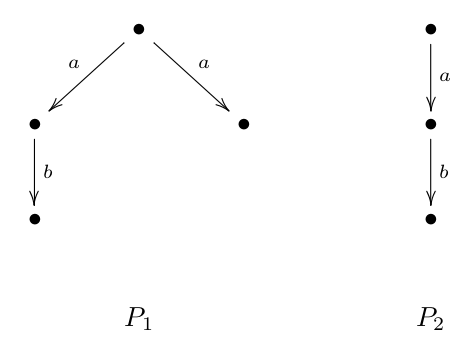
\includegraphics[width=0.5\linewidth]{images/nbisim-procs-ex1.png}
    \caption{}
    \label{fig:nbisim-procs-ex1}
\end{figure}

A process is often characterized by the sequence of actions it can perform, a view similar to classical automata theory where machines are identified by the strings they accept. However, this "trace" characterization is insufficient for bisimilarity. Consider the processes $P_1$ and $P_2$ illustrated in Figure \ref{fig:nbisim-procs-ex1}.

Although both can perform the sequence $a$ followed by $b$, they are not bisimilar. The difference lies in their branching structure:
\begin{itemize}
    \item $P_1$ can perform an action $a$ that leads to a state where no further action is possible, or it can perform $a$ followed by $b$. Thus, $P_1$ can perform $a$ not followed by any $b$.
    \item $P_2$, conversely, is more deterministic in its outcome; after every action $a$, it can always perform action $b$.  
\end{itemize}

\begin{figure}[ht]
    \centering
    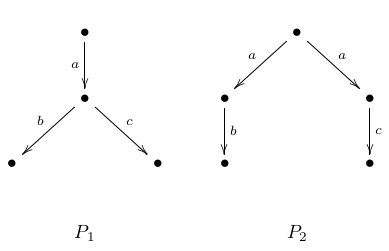
\includegraphics[width=0.5\linewidth]{images/nbisim-procs-ex2.png}
    \caption{}
    \label{fig:nbisim-procs-ex2}
\end{figure}

Because these two properties are complementary, they provide a formal ground to distinguish the two processes. A second example, shown in Figure \ref{fig:nbisim-procs-ex2}, further clarifies this distinction:
\begin{itemize}
    \item $P_1$ can perform an $a$ and then arrive at a state where it can choose between performing $b$ or $c$.
    \item $P_2$ makes the choice earlier; it can perform an $a$ that is only followed by $b$, or an $a$ that is only followed by $c$.
\end{itemize}

In this case, $P_1$ satisfies the property $\Diamond a (\Diamond b TT \wedge \Diamond c TT)$, meaning there exists an $a$-transition to a state where both $b$ and $c$ are possible. $P_2$ fails this property because after any $a$, it can only do $b$ or $c$, but not both.

\subsection{Syntax and Satisfiability}
To formalize these observations, we define a syntax for a logic often referred to as Hennessy-Milner logic. The language, denoted as Form, is generated by the following grammar:
\begin{equation*}
    \varphi := TT \mid \neg\varphi \mid \varphi_1 \wedge \varphi_2 \mid \Diamond a \varphi \hspace{0.5cm}\textit{where }a\textit{ is an action}
\end{equation*}
While the basic grammar uses binary conjunction, we often consider a more general form $\bigwedge_{i \in I} \varphi_i$, where $I$ is an indexing set that can potentially be infinite.

The satisfiability relation $\models \subseteq Proc \times Form$ determines when a process $P$ satisfies a formula $\varphi$ ($P\models\varphi \iff (P, \varphi)\in\models$). This relation is defined inductively: 
\begin{itemize}
    \item $P \models TT$ is always true for any process $P$.  
    \item $P \models \neg\varphi$ if and only if it is not the case that $P \models \varphi$.  
    \item $P \models \varphi_1 \wedge \varphi_2$ if and only if $P \models \varphi_1$ and $P \models \varphi_2$.  
    \item $P \models \Diamond a \varphi$ if and only if there exists a state $P'$ such that $P \xrightarrow{a} P'$ and $P' \models \varphi$.  
\end{itemize}

Other logical operators like $FF$ (false), disjunction ($\vee$), and implication ($\Rightarrow$) can be derived from these primitives. A particularly useful operator is the "box" operator. Let us define $\lnot\Diamond a\varphi$ as $\Box a\lnot \varphi$:
\begin{align*}
    P\models \Box a\varphi \iff P\models\lnot\Diamond a\lnot\varphi \iff P\not\models\Diamond a\lnot\varphi \iff\\
    \not\exists:P\xrightarrow{a}P'\land P'\models\lnot\varphi\iff \forall P':P\not\xrightarrow{a}P'\lor P'\models \varphi
\end{align*}
From the last condition, we have that $P\models\Box a \varphi$ if and only if
\begin{equation*}
    \forall P':P\xrightarrow{a}P'\Rightarrow P'\models\varphi
\end{equation*}

\begin{Example}{The formula $\Box a FF$}{}
    Let us consider the formula $\Box a FF$.
    By applying the definitions, $P \models \Box a FF$ if and only if for every $P'$ such that $P \xrightarrow{a} P'$, it holds that $P' \models FF$. However, since no process can ever satisfy $FF$, this condition can only be met if there are no such $P'$ states. Therefore, $P \models \Box a FF$ is true if and only if the process $P$ cannot perform action $a$.  
\end{Example}

It can be seen that for $\varphi\triangleq\Diamond a\Box b FF$ we have that $P_1\models\varphi$ whereas $P_2\not\models\varphi$ in Figure \ref{fig:nbisim-procs-ex1}. Instead, for $\varphi\triangleq\Box a\Diamond b TT$ and $\varphi\triangleq\Diamond a(\Diamond b TT \land \Diamond c TT)$ are both satisfied by $P_1$ but not $P_2$ in Figure \ref{fig:nbisim-procs-ex2}.

The fundamental link between logic and process equivalence is established by the following theorem. We define $L(P)$ as the set of all formulae satisfied by a process $P$
\begin{equation*}
    L(P) = \{\varphi\in Form : P \models \varphi\}
\end{equation*}

\begin{Thm}{$P\sim Q$ if and only if $L(P)=L(Q)$}{}\label{thm:PsimQ-iff-lPeqlQ}
The theorem states that two processes are bisimilar ($P \sim Q$) if and only if they satisfy the same set of formulae ($L(P) = L(Q)$).

By induction on the syntax tree of the formula, let us show that
\begin{equation*}
    \varphi\in L(P) \iff \varphi\in L(Q)
\end{equation*}

\begin{demonstration}\phantom{}
\begin{itemize}
    \item Base Case: For $\varphi = TT$, every process satisfies it, so $TT \in L(P)$ and $TT \in L(Q)$ holds trivially. 
    \item Inductive Step: We assume the property holds for trees of height $h$ and consider height $h+1$. Let us distinguish on the outmost operator in $\phi$:
    \begin{enumerate}
        \item For conjunction ($\varphi\triangleq\bigwedge_{i \in I} \varphi_i$), $P \models \varphi$ means $P \models \varphi_i$ for all $i$. 
        \begin{equation*}
            \varphi\in L(P)\iff P\models\varphi \iff \forall i\in I\textit{ }P\models \varphi_i \iff \forall i\in I\textit{ }\varphi_i\in L(P)
        \end{equation*}
        By definition, every formula $\varphi_i$ has a syntatic tree of height at most $h$; hence, by inductive hypothesis, $\varphi_i\in L(P)\iff \varphi_i\in L(Q)$, $Q \models \varphi_i$ for all $i$, so $Q \models \varphi$.
        \begin{equation*}
            \forall i\in I\textit{ }\varphi_i\in L(Q)\iff \forall i\in I\textit{ }Q\models\varphi_i\iff \bigwedge_{i\in I}p_i\in L(Q)\iff \varphi\in L(Q)
        \end{equation*}
        \item For negation ($\varphi\triangleq\neg \varphi'$), $\varphi \in L(P)$ implies $\lnot\varphi'\in L(P)$ that implies $\varphi' \notin L(P)$. The height of the syntax tree for $\varphi'$ is $h$; by the inductive hypothesis
        \begin{equation*}
            \varphi' \notin L(P)\iff \varphi'\notin L(Q)\iff\neg \varphi' \in L(Q)
        \end{equation*}
        \item For the diamond operator ($\varphi\triangleq\Diamond a \varphi'$), if $P \models \Diamond a \varphi'$, there is a $P \xrightarrow{a} P'$ with $P' \models \varphi'$. Since $P \sim Q$, there must be a $Q \xrightarrow{a} Q'$ such that $P' \sim Q'$. Because the height of the syntax tree for $\varphi'$ is $h$, by the inductive hypothesis, $Q' \models \varphi'$, which means $Q \models \Diamond a \varphi'$.
    \end{enumerate}
\end{itemize}

Up to now, we have proved that $\varphi\in L(P)\implies \varphi\in L(Q)$. To complete the proof, we have to prove the converse implication; this can be easily done by swapping $P$ and $Q$.
\end{demonstration}

Now we want to prove the other side of the $\iff$ theorem (i.e. $L(P)=L(Q)$  if and only if  $P\sim Q$). 
\begin{demonstration}
For this we can prove that $R\triangleq\{(P,Q):L(P)=L(Q)\}$ is a simulation; this suffices, since the relation just defined is trivially symmetric. 

Let $(P, Q)\in R$ and $P\xrightarrow{a} P$. Let us consider
\begin{equation*}
    \varphi\triangleq\Diamond a\varphi' \textit{ where }\varphi'\triangleq\bigwedge_{\varphi''\in L(P')}\varphi''
\end{equation*}
By construction, $P \models \varphi$, hence $Q \models \varphi$, because $L(Q) = L(P )$; then, $\exists Q' : Q \xrightarrow{a} Q'$ such that $Q'\models \varphi'$ . 

Hence, $\forall\varphi''\in L(P').\varphi'' \in L(Q')$, i.e. $L(P')\subseteq L(Q')$. 

By contradiction, let us assume that the inclusion is proper, i.e. $L(P')\subset L(Q')$. Thus, $\exists\varphi' : \varphi'\in L(Q')\land \varphi \notin L(P')$. 

Then, $\lnot\varphi'\in L(P')$ and this would imply that $\lnot\varphi'\in L(Q')$. This is a contradiction because $L(Q')$ cannot contain a formula and its negation.
\end{demonstration}
\end{Thm}

\subsection{Sub-logics}
While this logical approach is highly effective for proving inequivalence—requiring only a single formula satisfied by one process but not the other—it is less practical for proving equivalence. To show $P \sim Q$, one would theoretically need to check an infinite set of formulae, as $L(P)$ contains infinite variations like $TT, TT \wedge TT, \dots$. Even for simple processes, the action set may be infinite, leading to an infinite number of properties like $\Box b FF, \Box c FF$, etc.  
We can also explore sub-logics by removing certain operators to see what notions of equivalence they characterize:
\begin{enumerate}
    \item \textit{Negation-free Logic}\index{Negation-free Logic} ($L_\neg$): If we remove negation, the formula $\Box a FF$ is no longer expressible. We can only describe what a process can do. Theorem \ref{thm:PsimQ-iff-lPeqlQ} states that $P$ simulates $Q$ if and only if $L_\neg(Q) \subseteq L_\neg(P)$. Consequently, a double simulation exists between $P$ and $Q$ if and only if $L_\neg(P) = L_\neg(Q)$. In Figure \ref{fig:nbisim-procs-ex1}, $L_\neg(P_1) = L_\neg(P_2)$ because they simulate each other, even though they are not bisimilar.  
    \item \textit{Negation-and Conjunction-free Logic}\index{Negation-and Conjunction-free Logic}: Removing both negation and conjunction results in a logic that characterizes trace equivalence. In this sub-logic, $L(P) = L(Q)$ if and only if the processes accept the same set of strings (traces). For instance, $P_1$ and $P_2$ from Figure \ref{fig:nbisim-procs-ex2} are trace equivalent and thus satisfy the same formulae in this restricted logic.  
\end{enumerate}

A similar logic exists for weak bisimilarity, where the standard diamond operator $\Diamond a$ is replaced by $\ll a \gg$.
\begin{equation*}
    \varphi := TT \mid \neg\varphi \mid \varphi_1 \wedge \varphi_2 \mid \ll\gg a \varphi \hspace{0.5cm}\textit{where }a\textit{ is an action}
\end{equation*}
This operator accounts for internal $\tau$ actions, such that $P \models \ll a \gg \varphi$ if and only if exists a $P'$ such that $P \xRightarrow{\widehat{a}} P'$ and $P' \models \varphi$ .  

\section{Algorithmic Approach to Bisimilarity}
Establishing bisimilarity between two states in a Labelled Transition System (LTS) is fundamentally a problem of classification. When dealing with finite-state systems, we can determine if two states are bisimilar by treating the problem as a special case of the \textit{Relational Coarsest Partition Problem} (RCPP)\index{Relational Coarsest Partition Problem}. The core objective of RCPP is to refine a set of elements into distinct classes, or "blocks," by starting from the most inclusive perspective and gradually separating elements that fail to meet a specific equivalence criterion.

The RCPP methodology follows a "top-down" refinement logic. We begin with the coarsest possible partition, which is simply the set $S$ containing all states of the LTS. From there, we iteratively apply a splitting rule to break these blocks into smaller sub-blocks. This process continues until no further splits are possible—a state known as a stable partition. At the conclusion of the algorithm, two states are considered to be in the target relation (in this case, bisimilar) if and only if they remain in the same block.

The specific nature of the equivalence we are checking is entirely defined by the splitting rule used. For bisimilarity, this rule ensures that states are separated if they cannot match each other's transitions in a way that leads to equivalent future states.

To understand how blocks are divided, let $B$ be a generic block within a partition, and let $s$ and $t$ be two states belonging to that block. We define $block(s)$ as the set of all states currently residing in the same block as $s$. Under the standard definition of bisimilarity, $s$ and $t$ must be separated into different blocks if one can perform an action that the other cannot, or if they reach states that are no longer considered equivalent in the current partition:
\begin{equation*}
    \exists\alpha, s'\textit{ s.t. }s\xrightarrow{\alpha}s'\land\forall t'(t\not\xrightarrow{\alpha}t'\lor t'\notin block(s'))
\end{equation*}

To implement this efficiently, we use an alternative but equivalent condition based on the set of reachable blocks. We define:
\begin{equation*}
    tgt_{\alpha}(s) \triangleq \{B' : \exists s' \text{ such that } s \xrightarrow{\alpha} s' \wedge s' \in B'\}
\end{equation*}

This set, $tgt_{\alpha}(s)$, contains all the blocks reachable from state $s$ via a transition labeled with the action $\alpha$. Consequently, the splitting condition becomes straightforward: two states $s$ and $t$ must be split if there exists some action $\alpha$ such that the blocks they can reach are not identical:
\begin{equation*}
    \exists \alpha : tgt_{\alpha}(s) \neq tgt_{\alpha}(t)
\end{equation*}

Essentially, if $s$ can reach a certain "type" of state (a specific block) with action $\alpha$ and $t$ cannot, they are not bisimilar and cannot remain in the same block.

\begin{lstlisting}[mathescape, caption={RCPP algorithm.}, captionpos=b]
    INPUT: LTS=(S,$\Lambda$,$\rightarrow$) ; s,t $\in$ S
    
          P $\leftarrow$ {S}
    LOOP: forall B $\in$ P do
              forall $\alpha\in\Lambda$ do
                  I $\leftarrow$ split(B, $\alpha$, P)
                  if I $\neq$ {B} then
                      P $\leftarrow$ (P \ {B}) $\cup$ I
                      goto LOOP
          forall B $\in$ P do
              if {s,t} $\subseteq$ B then return true
          return false
\end{lstlisting}

The Main Algorithm (often referred to as the Kanellakis-Smolka algorithm) takes an LTS and two states, $s$ and $t$, as input. 
It initializes the partition $\mathcal{P}$ to contain a single block $\{S\}$. The algorithm then enters a loop:
\begin{enumerate}
    \item For every block $B$ in the current partition $\mathcal{P}$ and every possible action $\alpha$ in the set of labels $\Lambda$, it attempts to split the block. 
    \item The \texttt{split(B, $\alpha$, P)} function is called.
    \item If the function returns a new set of sub-blocks (meaning $B$ was not stable), the old block $B$ is removed from $\mathcal{P}$, the new sub-blocks are added, and the algorithm restarts the loop to ensure consistency.  
    \item Once no more splits can be made, the algorithm checks if the input states $s$ and $t$ are in the same block. If they are, it returns true; otherwise, it returns false.  
\end{enumerate}

\begin{lstlisting}[mathescape, caption={Split algorithm.}, captionpos=b]
    INPUT: (B,$\alpha$,P)
    
    choose s $\in$ B
    B1 $\leftarrow\emptyset$ B2 $\leftarrow\emptyset$
    forall t $\in$ B do
        if tgt$_\alpha$(s) = tgt$_\alpha$(t) then B1 $\leftarrow$ B1 $\cup$ {t}
                             else B2 $\leftarrow$ B2 $\cup$ {t}
    if B2 = $\emptyset$ then return {B}
               else return {B1, B2}
\end{lstlisting}

The Splitting Algorithm itself works by picking a reference state $s$ within block $B$. It then iterates through every other state $t$ in that same block. If $t$ has the exact same transition targets as $s$ for the action $\alpha$ (meaning $tgt_{\alpha}(s) = tgt_{\alpha}(t)$), it is placed in sub-block $B_1$. If the targets differ, $t$ is moved to $B_2$. If $B_2$ ends up empty, no split occurred; otherwise, the block $B$ is successfully partitioned into $B_1$ and $B_2$.  

\begin{Example}{RCPP algorithm}{}
    To illustrate this, consider two processes: $P_1 \triangleq a|\bar{a}$ and $P_2 \triangleq a\bar{a} + \bar{a}a + \tau$.

    \begin{minipage}{0.5\textwidth}
        \centering
        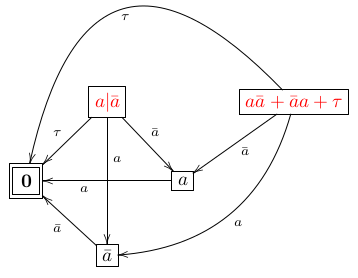
\includegraphics[width=1\linewidth]{images/rcpp-example.png}
        %\captionof{figure}{}
    \end{minipage}
     \begin{minipage}{0.5\textwidth}
        \centering
        \begin{tabular}{|c|c|}
            \hline
             Assigned Value & State\\\hline
             1 & $a|\bar{a}$\\\hline
             2 & $a\bar{a} + \bar{a}a + \tau$\\\hline
             3 & $\bar{a}$\\\hline
             4 & $a$\\\hline
             5 & 0\\\hline
        \end{tabular}
    \end{minipage}

    We assign numerical values to the states for clarity: $1$ for $P_1$, $2$ for $P_2$, $3$ for $a$, $4$ for $\bar{a}$, and $5$ for the terminated state $0$.

    \begin{enumerate}
        \item Initial State: $\mathcal{P} = \{\{1, 2, 3, 4, 5\}\}$.
        \begin{itemize}
            \item We choose action $a$ and block $B = \{1, 2, 3, 4, 5\}$.
            \item Here, $tgt_a(1) = \{B\}$, $tgt_a(2) = \{B\}$, and $tgt_a(4) = \{B\}$ (because they can all perform $a$ to reach a state in the current universal block). However, states $3$ and $5$ cannot perform action $a$, so $tgt_a(3) = \emptyset$ and $tgt_a(5) = \emptyset$.  
            \item Result: $B$ is split into $\{1, 2, 4\}$ and $\{3, 5\}$.  
        \end{itemize}
        \item Second Refinement: $\mathcal{P} = \{\{1, 2, 4\}, \{3, 5\}\}$.
        \begin{itemize}
            \item We choose action $\bar{a}$ and block $B = \{1, 2, 4\}$.
            \item States $1$ and $2$ can perform $\bar{a}$ to reach states in existing blocks, so $tgt_{\bar{a}}(1) = tgt_{\bar{a}}(2) = \{B\}$. State $4$, however, cannot perform $\bar{a}$, so $tgt_{\bar{a}}(4) = \emptyset$.  
            \item Result: Block $\{1, 2, 4\}$ is split, leading to $\mathcal{P} = \{\{1, 2\}, \{4\}, \{3, 5\}\}$.  
        \end{itemize}
        \item Third Refinement:
        \begin{itemize}
            \item We choose action $\bar{a}$ and block $B = \{3, 5\}$.
            \item State $3$ can perform $\bar{a}$ ($tgt_{\bar{a}}(3) = \{B\}$), but state $5$ cannot ($tgt_{\bar{a}}(5) = \emptyset$).  
            \item Result: $\mathcal{P} = \{\{1, 2\}, \{4\}, \{3\}, \{5\}\}$.  
        \end{itemize}
        
        At this stage, no further actions or blocks will cause a split. Since states $1$ and $2$ remain together in the same block, we conclude that $a|\bar{a}$ and $a\bar{a} + \bar{a}a + \tau$ are bisimilar.  
    \end{enumerate}

    The algorithm is equally effective at proving states are not equivalent. Consider $P_1 \triangleq a|\bar{a}$ and $P_2 \triangleq a\bar{a} + \bar{a}a$ (notably excluding the $\tau$ transition).  

    Initially, the partitioning might proceed similarly until we reach $\mathcal{P} = \{\{1, 2\}, \{4\}, \{3\}, \{5\}\}$. However, if we then examine the $\tau$ action for the block $\{1, 2\}$, we find a discrepancy. Process $P_1$ ($a|\bar{a}$) can perform a $\tau$ transition (an internal communication between $a$ and $\bar{a}$), whereas the version of $P_2$ without the explicit $+\tau$ term cannot. Because $tgt_{\tau}(1) \neq tgt_{\tau}(2)$, the block $\{1, 2\}$ would be split into $\{1\}$ and $\{2\}$. Since they end up in different blocks, the processes are not bisimilar
\end{Example}

\subsection{Correctness of the Algorithm}
The reliability of any algorithmic approach depends on its termination and the correctness of its output. For the Kanellakis-Smolka algorithm, termination is guaranteed by the finite nature of the Labelled Transition System (LTS). Since every iteration of the refinement cycle operates on a finite number of states and transitions, and the partition $\mathcal{P}$ can have a maximum cardinality of $|S|$ (where each state resides in its own individual block), there is a physical limit to how many times a block can be split. Once the partition reaches a state where no block can be further subdivided according to the splitting rule, the algorithm must terminate.

\begin{Thm}{$s\sim t\iff \exists B\in P_f$ $\{s, t\}\subseteq B$}{}
    The algorithm effectively decides bisimilarity ($s \sim t$) by checking if the two states belong to the same block in the final partition $\mathcal{P}_f$. This is proven through two logical directions:
    The "If" direction (Completeness) and the the "Only If" direction (Soundness)
\begin{demonstration}
    We must show that if two states are bisimilar ($s \sim t$), they will necessarily remain in the same block in the final partition. This is often proven by contradiction. Suppose $s$ and $t$ are found in different blocks $B_j'$ and $B_j''$ at the end of the process. At the start of the algorithm, all states were together in a single block. If $s$ and $t$ were separated at some step $(i+1)$, there must have existed an action $\alpha$ such that their target sets were different, meaning $tgt_{\alpha}(s) \neq tgt_{\alpha}(t)$. Specifically, this would mean one state can reach a block that the other cannot reach with the same action. Because blocks represent equivalence classes at that stage of the algorithm, this difference in reachability contradicts the initial assumption that $s \sim t$.
\end{demonstration}
\begin{demonstration}
    We must also show that if two states $s$ and $t$ are in the same block of $\mathcal{P}_f$, they are truly bisimilar. To prove this, we define a relation $R$ where $(x, y) \in R$ if and only if $x$ and $y$ share the same block in $\mathcal{P}_f$. By construction, $(s, t) \in R$. Because the algorithm has terminated, the blocks are "stable," meaning for any $(x, y) \in R$ and any transition $x \xrightarrow{\alpha} x'$, there must be a matching $tgt_{\alpha}(x) = tgt_{\alpha}(y)$. This ensures there is some $y \xrightarrow{\alpha} y'$ such that $x'$ and $y'$ are in the same block, thereby maintaining $(x', y') \in R$. Since $R$ is symmetric and satisfies the simulation property, it is a bisimulation, proving $s \sim t$.
\end{demonstration}
\end{Thm}

\subsection{Complexity Analysis of the Algorithm}
The efficiency of this algorithm is a significant improvement over exponential methods like powerset construction. Let the LTS be defined by $n$ states and $m$ transitions. The computational cost can be broken down as follows:
\begin{itemize}
    \item The "goto" instruction, which restarts the refinement process, is triggered only when a block is successfully split. In the worst-case scenario, we split only one state at a time into its own block, meaning this can happen at most $O(n)$ times.
    \item Within the main loop, we iterate through every block $B$ and every action $\alpha$. The core cost lies in the split function, which examines every state $t$ in the block and checks the condition $tgt_{\alpha}(s) = tgt_{\alpha}(t)$.
    \item The total work done in these nested loops across the entire algorithm is proportional to the number of transitions. By analyzing every $\alpha$-transition from states in a block exactly once during a refinement step, the inner logic scales with $m$:
    \begin{equation*}
        \sum_{B\in\mathcal{P}}\sum_{a\in\Lambda}\sum_{t\in B}|\{t':t\xrightarrow{\alpha}t'\}|=
        \sum_{B\in\mathcal{P}}\sum_{t\in B}\sum_{a\in\Lambda}|\{t':t\xrightarrow{\alpha}t'\}|=
        \sum_{t\in S}\sum_{a\in\Lambda}|\{t':t\xrightarrow{\alpha}t'\}|= |\rightarrow| = m
    \end{equation*}
\end{itemize}
Combining the $O(n)$ refinement steps with the $O(m)$ work per step (using proper data structures), the overall complexity of the algorithm is $O(nm)$.

\subsection{Efficiently Handling Blocks}
To achieve $O(nm)$ complexity, the algorithm requires a sophisticated way to manage and compare blocks. This is done through a symbolic representation where every block is associated with a unique binary string index.
\begin{itemize}
    \item \textit{Index Creation:} The initial block $S$ is assigned the index "0". Whenever a block is split, its children inherit the original string with an additional bit—"0" for the first sub-block and "1" for the second. For example, if $S = \{1, 2, 3, 4, 5\}$ is split into $B_1 = \{1, 2, 4\}$ and $B_2 = \{3, 5\}$, their indices become "00" and "01" respectively.  If then $B_2$ is split into $B_3 = \{3\}, B_4 = \{5\})$, then the associated strings will be "010" for $B_3$ and "011" for $B_4$.
    \item \textit{Transition Matrix:} Transitions are stored as triples $(s, \alpha, \sigma)$, where $\sigma$ is the binary index of the block containing the target state. By ordering these triples lexicographically based on states and actions, we can find and compare target sets quickly. While the initial ordering costs $O(m \log m)$, updates to the indices during splits do not require a full re-sort.

    For example, suppose that we start with this matrix representation:
    \begin{align*}
        &\ldots\\
        &(s_1, \alpha_1, 00)\\
        &(s_1, \alpha_2, 01)\\
        &(s_1, \alpha_2, 11)\\
        &\ldots
    \end{align*}
    If we split "01" (into "010" and "011"), wherever $s_1$ has to go, the matrix will be:
    \begin{align*}
        &\ldots\\
        &(s_1, \alpha_1, 00)\\
        &(s_1, \alpha_2, 01b)\\
        &(s_1, \alpha_2, 11)\\
        &\ldots
    \end{align*}
\end{itemize}

When executing \texttt{split(B, $\alpha$, $\mathcal{P}$)}, we choose a pivot state $s \in B$ to serve as the benchmark. The comparison of $tgt_{\alpha}(s)$ and $tgt_{\alpha}(t)$ for all other states $t$ in the block follows these rules:  
\begin{enumerate}
    \item If the pivot $s$ has no $\alpha$-transitions ($k=0$), we simply split the block into states that also have no $\alpha$-transitions ($B_1$) and those that do ($B_2$).  
    \item If $s$ has $\alpha$-transitions, we look at the index $\sigma$ of its first $\alpha$-transition. Any state $t$ whose first $\alpha$-transition leads to a block with a different index is immediately moved to $B_2$.  
    \item We repeat this for the second, third, and $k$-th transitions of the pivot. If at any point a state $t$ lacks a matching transition or points to a different block index, it is moved to $B_2$.  
    \item After checking all transitions of the pivot, any state $t$ that has additional $\alpha$-transitions beyond those matched with the pivot is moved to $B_2$, as its $tgt_{\alpha}$ set is necessarily larger and thus different.
\end{enumerate}
